\chapter{Introduction}
\label{ch:Intro}
\par
One of the recurring motifs throughout this thesis is how recent advances in computer
hardware and reduced cost of computations helped us push the boundaries of physical
knowledge. Our exploration starts with one of the most widely used numerical tools in any computational discipline, the Monte Carlo (MC) method. Because of the use
of random numbers, these methods are believed to carry the name after the most
famous casino in the world, Monte Carlo Casino in Monaco. The term \textit{Monte Carlo} was
first used in modern literature by S. Ulam, E. Fermi, J. von Neumann, and N.
Metropolis while they were working on the Manhattan Project in Los Alamos National
Laboratory during the second world war. MC methods will also play a significant role in this
thesis as one of the primary tools for analyzing physical systems. Our
journey will start with an exploration of different realizations of gauge lattice models;
we will introduce simple Wegner Ising gauge theory, the fundamental block, and later
build upon it by adding matter fields to the lattice. MC played a significant role in
the early days of lattice gauge theories helping us advance our understanding of the theory of
elementary particles. We will use it similarly to explore phase diagrams and
phase transitions in our lattice gauge models. On the next stop, we will explore how closed, unitary quantum systems can (appear to) thermalize, a question
that has been at the heart of statistical physics for a long time. The final stop will
be one governed by the recent advances of machine learning in areas of physics.
We will try to quantify the multipartite entanglement in quantum systems by combining MC simulations and newly proposed variational wave functions in the form
of restricted Boltzmann machines (RBM). Some of the problems, or quirks, of MC methods
can also appear in the modern training of neural networks. Most prominent is
the choice of initial distribution for parameters we are trying to optimize. Using statistical physics and field theory tools, we will find optimal initial conditions to improve neural networks' training speed and accuracy.
\newpage     
\section{Statistical physics}
\label{sec:statPhys}
The primary goal of statistical physics is an exploration of macroscopic quantities and the calculation thereof. Often, the systems we explore are made up of many degrees of freedom, and solving them exactly is impossible. In order to do this, we will assume that the statistical average over all possible states can replace the time average. 
\par 
One of the main assumptions we make when resorting to statistical calculations instead of fully dynamically solving the system is the principle of \textit{ergodicity}. Ergodicity states that if the system is left to evolve, all accessible states will eventually be realized. This assumption helps us often turn insolvable time integrals into relatively easy and, more importantly, simulation-friendly integrals over the probability distributions of those states. For example, let us say we want to study some volume of gas in a container. At standard temperature and pressure, one liter of oxygen contains around $3\cdot 10^{22}$ oxygen molecules moving around the container. Just writing down equations of motion for all molecules would take a very long time, but no practical conclusion can be drawn even if we manage to do it. Hence we turn to the methods of statistical physics.
\par
These statistical integrals are averaging over many system realizations while keeping certain parameters fixed. These sets of systems with specific parameters fixed are called \textit{ensembles}. For example, a glass of water sitting on a counter at a fixed temperature will have many different configurations of water molecules that fluctuate while having a fixed \textit{average} energy.
\par
There are several well-known ensembles according to corresponding fixed quantities. If the fixed quantity is energy, the ensemble is called \textit{microcanonical}, we can denote the total number of states with that energy as $\mathcal{N}(E)$, the probability that any of those instances are realized is $\frac{1}{\mathcal{N}(E)}$ and the probability that system is in some other energy $E^\prime \neq E$ is simply zero.
\par
Now we can define the \textit{entropy} of a system as:
\begin{equation}
	S(E) = k_B \log \mathcal{N}(E) \mathperiod
\end{equation}
Because the number of states in a system of $N$ bits/particles is of order $\mathcal{N}(E) \sim 2^N$, it follows that the entropy is proportional to a number of particles in the system $S(E) \sim N$. We can see that this makes entropy an extensive quantity. For two non-interacting systems at energies $E_1$ and $E_2$, we get the total number of states in both systems as:
\begin{equation*}
	\mathcal{N}(E_1, E_2) = \mathcal{N}(E_1)\mathcal{N}(E_2) \mathcomma
\end{equation*}
and the entropy will be: 
\begin{equation*}
	S(E_1, E_2) = S(E_1) + S(E_2) \mathperiod
\end{equation*}
\par
Often systems are not isolated but actually in contact with some reservoir at a specific temperature $T$. One way we can remedy this is by including the reservoir in our calculation and using a microcanonical ensemble, but doing this results in very complex calculations and, more importantly, properties of the reservoir that are often not of interest to us. Because of this, we will introduce an ensemble at a fixed temperature called \textit{canonical}. Now the system can be in states with the different energy that will fluctuate around some well-defined average value. The average energy of the system is defined as a sum of energies of all the states weighted with their respective probabilities:
\begin{equation}
	\langle E \rangle = \sum_i p_i E_i \  .
	\label{eq:averageenergy}
\end{equation}
Here $p_i$ is a probability that the system is in the state with energy $E_i$. One can derive, either by entropy maximization or placing the system in contact with a heat bath, that a system with only energy as conserved quantity has a probability, also known as \textit{Boltzmann distribution}:
\begin{equation}
	p_i = \frac{\exp(-\beta E_i)}{\sum_i \exp(-\beta E_i)} \mathperiod
	\label{eq:canonicalprob}
\end{equation}
We have introduced a factor, inverse temperature, $\beta=\frac{1}{k_B T}$ where $k_B$ is Boltzman constant $=1.380649 \cdot 10^{-23} \text{J}\cdot\text{K}^{-1}$, and $T$ temperature of the ensemble. Exponential factors ensure that states with energies $E_i \gg k_B T$ get suppressed while states with $E_i \leq k_B T$ have a chance of being populated. We can check that this makes sense. Let $T \rightarrow 0$, and the system is forced to a ground state energy with all higher states being suppressed. We can also define the entropy for the canonical ensemble as follows:
\begin{equation}
	S = -k_B \sum_i p_i \log p_i \mathperiod
\end{equation} 
The normalization factor is an essential quantity in Eq.(\ref{eq:canonicalprob}). This sum over all accessible states that ensure that probability sums to $1$ is called \textit{partition function}:
\begin{equation}
	Z = \sum_i \exp(-\beta E_i) \mathperiod
\end{equation}
Once we know the partition function, we can compute any quantity about the system; we have complete knowledge. Let us explore what information we can extract from the partition function. We can define the free energy at fixed temperature as:
\begin{equation}
	F = \langle E \rangle - TS \mathcomma
\end{equation}
where $T$ is temperature and $S$ is entropy. We can think of free energy as energy available to the system, an intricate interplay between internal energy and entropy. At the fixed temperature, we can get free energy directly from the partition function:
\begin{equation}
	F = -k_B T \log Z \mathperiod
\end{equation}
To connect average energy and a partition function, we can plug Eq.(\ref{eq:canonicalprob}) into Eq.(\ref{eq:averageenergy}):
\begin{equation*}
	\langle E \rangle = \sum_i p_i E_i = \sum_i \frac{E_i \exp(-\beta E_i)}{Z} \mathperiod
\end{equation*}
However, this can be rewritten in the form of a partial derivative of the partition function:
\begin{equation}
	\langle E \rangle = \pdv{\beta} \log Z \mathperiod
\end{equation}
As stated earlier, energy is not constant in the canonical ensemble but fluctuates. The exponential factor in Boltzmann distribution ensures that these fluctuations are around $k_B T$; we can compute them as a variance of energy:
\begin{equation*}
	\sigma^2_E = \langle (E - \langle E \rangle)^2 \rangle = \langle E^2 \rangle - \langle E \rangle^2 = \pdv[2]{\beta} \log Z = - \pdv{\langle E \rangle}{\beta} \mathperiod
\end{equation*} 
We can make a connection with specific heat that will give us a different interpretation of these fluctuations. Specific heat is a thermodynamic quantity defined as $C = \pdv{E}{T}$ or how much the energy of a system changes as we vary the temperature. Specific heat can be measured while we keep other parameters fixed, like volume or pressure. So, for example, specific heat at fixed volume will be $C_V = \pdv{E}{T}\bigg\rvert_{V=\text{const}}$. Now we can connect specific heat and the variance of energy:
\begin{equation*}
	\sigma^2_E = k_B T^2 C_V \mathperiod
\end{equation*}
Interesting conclusions can be drawn from here; if $C_V$ of the system is large, it can easily absorb bigger energy fluctuations without changing its temperature. Another conclusion is that for macroscopic systems ($N \gg 1$) away from the critical point, $E \propto N$ and $C_V \propto N$, so we have that energy fluctuations scale as:
\begin{equation}
	\frac{\sigma_E}{E} \sim \frac{1}{\sqrt{N}} \mathperiod
\end{equation}
In the limit, when $N \rightarrow \infty$, the energy becomes exactly $\langle E \rangle$. This is also known as a \textit{thermodynamic limit}. These fluctuations are too small for real systems to be detected, but they are often how we calculate thermodynamic quantities in simulations.
\par
The question now is what happens with the fluctuations of other quantities. If there are terms in the Hamiltonian $\mathcal{H}$, of form $-XY$, where $Y$ is some field and $X$ conjugate variable to which field $Y$ is coupled then we have:
\begin{equation}
	\langle X \rangle = \frac{1}{\beta Z} \pdv{Y} \sum_i \exp(-\beta \mel{i}{\mathcal{H}}{i}) = -\pdv{F}{Y} \mathperiod
\end{equation}
Now $\mel{i}{\mathcal{H}}{i}$ contains the term of form $-XY$ on which partial derivative acts. So if we desire to find an average value of any conjugate variable, we need to differentiate free energy with respect to the appropriate coupled field. If there is no term coupling field to desired quantity, we can add it, find the derivative, and later set the same field to zero, restoring an original Hamiltonian. Doing further differentiation, we can see that:
\begin{equation}
	-\frac{1}{\beta}\pdv[2]{F}{Y} = \frac{1}{\beta} \pdv{\langle X \rangle}{Y} = \langle X^2 \rangle - \langle X \rangle^2 \mathperiod
	\label{eq:generalvariance}
\end{equation}
We used this variance to connect energy fluctuations to the specific heat. Now we have a general way of finding these variances from the second derivatives of free energy with respect to coupled fields. The derivative in Eq.(\ref{eq:generalvariance}) measures the magnitude of the response of $X$ to changes happening in $Y$. This is called \textit{susceptibility} of $X$ to $Y$ and is usually written as $\chi$. This gives us a general way of calculating susceptibility directly from the simulations by measuring fluctuations in desired quantities. A practical example of susceptibility that will be important to us is the magnetic susceptibility or how total magnetization of the system changes as we vary the external magnetic field.
\par
Some systems can go through a \textit{phase transition}, a sudden change in a system's specific property, becoming discontinuous in the large $N$ limit. The prominent feature of a phase transition is the appearance of a non-vanishing value of \textit{order parameter}, some quantity that is non-zero in the ordered phase and then identically zero in the disordered phase. Different order parameters are identified in different systems; for example, in a ferromagnet, it is a spontaneous magnetization, and in the liquid-gas phase, it is the difference in the density between the liquid and gas phases at the transition line. They can be scalar or multi-component quantities as well. 
\par
The classification of phase transitions can be done by the order of discontinuous derivative of a free energy. If the first derivative of the free energy shows discontinuous behavior, we call those transitions \textit{first order}. If, on the other hand, the first order is continuous but the second derivative is not, we label those transitions \textit{second order}.
\par
We can deduce some qualitative characteristics of a model using \textit{Landau theory of phase transitions}. The main idea revolves around expanding the free energy in the powers of the order parameter. For this expansion to converge, we have to keep the order parameter small, so near the critical point. The Ising model in an external magnetic field $h$ is a popular toy system to illustrate the main concepts. The energy of the Ising model can be expressed as:
\begin{equation}
	E = -J \sum_{\langle i j \rangle} s_i s_j - h \sum_i s_i \mathcomma
	\label{eq:classicIsing}
\end{equation}
where spins $s_i \in \{-1,1\}$ and we sum over all neighboring sites $\langle i j \rangle$ in a $d$-dimensional hyper-cubic lattice.
\par
Let us start with the description of a second-order phase transition. Consider a general model (like the Ising case defined above) and denote an order parameter $m$ (in our case, total magnetization). Then we can expand the free energy as:
\begin{equation}
	F(T,m) = F_0 (T) + a(T) m^2 + b(T) m^4 + \cdots \mathperiod
	\label{eq:landauexpansion}
\end{equation}
We do not have odd terms because the theory is invariant under the change $m\rightarrow -m$, which forbids odd terms in the free energy (in our case, when $h=0$ Ising has this symmetry). The system's state can be found by extremizing the free energy, $\pdv{F}{m}=0$. We can immediately see that result will depend on the signs of the temperature-dependent terms. These terms can change sign with varying temperature as well. For simplicity, we will assume that $b(T) > 0$ for all $T$. If we do not impose this condition and let $b(T)$ have any sign, then we need to include higher terms of expansion ($m^6$ in our case) which can lead to the formation of tri-critical points, a phenomenon explored in the later chapters. In order to illustrate this further, we will use the free energy of the Ising model that we can calculate from mean-field theory\cite{sachdev_2011}:
\begin{equation}
	F = -\frac{1}{\beta}\log Z = \frac{1}{2}JNqm^2 - \frac{N}{\beta}\log(2\cosh \beta h_{\text{eff}}) \mathcomma
\end{equation}
where $q=2d$ is the number of nearest neighbors and $h_{\text{eff}} = h + Jqm$ is an effective (mean-field) magnetic field. We can expand this mean-field expression in order to compare coefficients with our free energy expansion:
\begin{equation}
	F(T,m) = -Nk_BT\log 2 + \left( \frac{NJq}{2}(1-Jq\beta) \right)m^2 + \left( \frac{N\beta^3J^4q^4}{12} \right) m^4 + \cdots \mathperiod
	\label{eq:freeEnergySecondOrder}
\end{equation}
The first term is just an additive constant, which will vanish once we take a derivative with respect to $m$. Consider then the quadratic term with coefficient $a(T)=\frac{NJq}{2}(1-Jq\beta)$ there are two different cases $a(T) > 0$ and $a(T) < 0$. From the expression of $a(T)=0$, we can also determine the critical temperature $T_c = \frac{Jq}{k_B}$. In the case of $a(T) > 0; T > T_c$, and thus when temperatures are high, we see that the only equilibrium solution is for $m=0$. On the other hand, when $T < T_c$, for low temperature, there are three solutions, $0, \pm \sqrt{-\frac{a(T)}{2b(T)}}$. Substituting these values in Eq.(\ref{eq:freeEnergySecondOrder}), we see that the free energy of a state with $m=0$ is higher than the other two and represents an unstable solution, Fig.(\ref{gr:secondOrderLandau}). We thus find that the free energy equals:
\begin{equation}
	F(T) = \begin{cases}
		F_0(T) & T > T_c \\
		F_0(T) - \frac{a(T)^2}{4b(T)^2} & T < T_c
	\end{cases} \mathperiod
\end{equation}
The important point is that if $a(T)$ is a smooth function, then the equilibrium value of $m$ also changes continuously from $m=0$ in the $T>T_c$ regime to a $m\neq0$ in a $T<T_c$ regime. We can also see that the free energy is continuous at the transition. However, suppose we differentiate free energy twice to get a specific heat. In that case, we will have a term $\frac{a(T)^{\prime2}}{b(T)}$ which is usually not equal to zero, and hence specific heat has a discontinuous change at $T=T_c$, defining characteristics of a second order phase transition.
\par
When we were expanding the free energy in Eq.(\ref{eq:landauexpansion}), we said that odd terms are forbidden by the symmetry $m\rightarrow-m$, so-called $\mathbf{Z}_2$ symmetry. Then when we found the equilibrium values of $m$ for $T<T_c$, we saw that the system had to choose one ground state of the two, $\pm \sqrt{-\frac{a(T)}{2b(T)}}$, this is the well-known phenomena of \textit{spontaneous symmetry breaking}. The Ising model discussion above illustrates how it is tied to the second-order phase transition.
\begin{figure}[H]
	\centering
	\begin{subfigure}{0.5\textwidth}
		\centering
		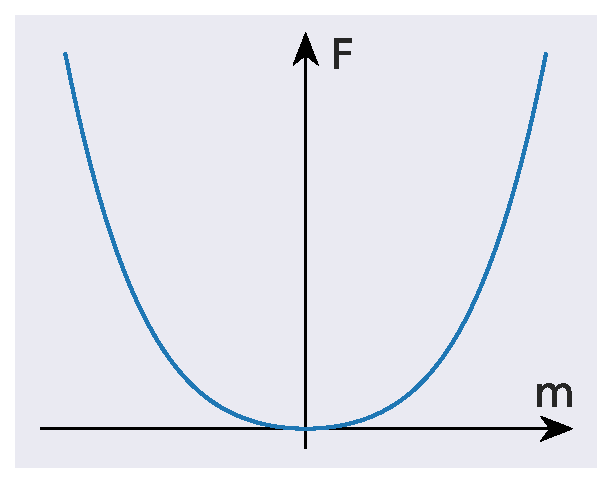
\includegraphics[width=0.8\columnwidth]{figures/introduction/secondOrder-a-positive.pdf}
	\end{subfigure}%
	\begin{subfigure}{0.5\textwidth}
		\centering
		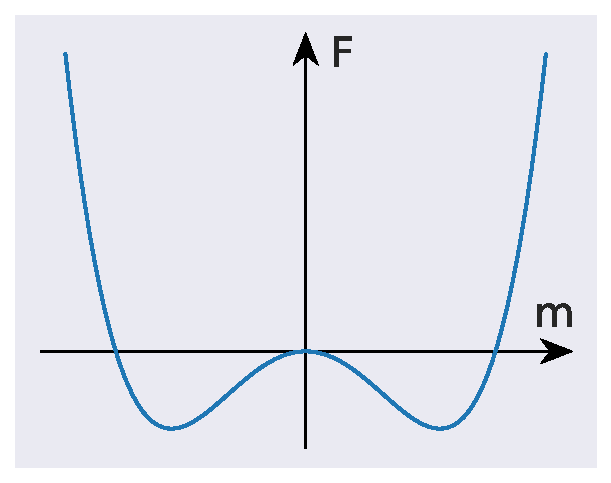
\includegraphics[width=0.8\columnwidth]{figures/introduction/secondOrder-a-negative.pdf}
	\end{subfigure}
	\caption{Free energy curves in the case of second-order phase transition. In the left graph, when $a(T)>0$, we see only one equilibrium solution at $m=0$. On the other hand, when $a(T)<0$ (right graph), two more solutions appear. The previously stable solution at $m=0$ now becomes unstable. We can see that the system can choose which stable solution to be in, which is what we call spontaneous symmetry breaking.}
	\label{gr:secondOrderLandau}
\end{figure}
\par
Let us briefly explore what happens when we include odd power terms of the order parameter in our expansion of the free energy $F$.
\begin{equation}
	F(T,m) = F_0(T) + \alpha(T)m + a(T)m^2 + \gamma(T)m^3 + b(T)m^4 + \cdots \mathperiod
	\label{eq:landauexpansionodd}
\end{equation}
If we look back at our definition of Ising model Eq.(\ref{eq:classicIsing}) we see that for $h\neq 0$ the system doesn't have $\mathbf{Z}_2$ symmetry in $m \rightarrow -m$, so we can use the expansion above:
\begin{equation}
	F(T,m) = -Nk_BT\log 2 + \frac{JNq}{2}m^2 - \frac{N}{2k_BT}(B+Jqm)^2 + \frac{N}{24(k_BT)^3}(B + Jqm)^4 + \cdots \mathperiod
\end{equation}
We will use the same assumption again that $b(T) > 0$ for all $T$. In the regime where $T<T_c$, we again have three solutions, but now the curve is skewed, and more importantly, two minima are no longer degenerate. An introduction of the external magnetic field $h$ broke the degeneracy that was initially there, and the other solution is called a meta-stable state. When odd terms in the expression for the free energy, $\alpha(T)$ and $\gamma(T)$, change signs, the curve goes from the left to the right picture in Fig.(\ref{gr:firstOrderLandau}). This changes the true ground state, and the transition from this new meta-stable state to the true ground state with lower energy is the first-order phase transition. In the example of the Ising model, this transition occurs when the external magnetic field $h$ changes sign. If we increase the temperature above the critical $T>T_c$, the free energy curve looks similar to the second-order transition. However, it is shifted because of the linear term $\alpha(T)$.
\begin{figure}[H]
	\centering
	\begin{subfigure}{0.33\textwidth}
		\centering
		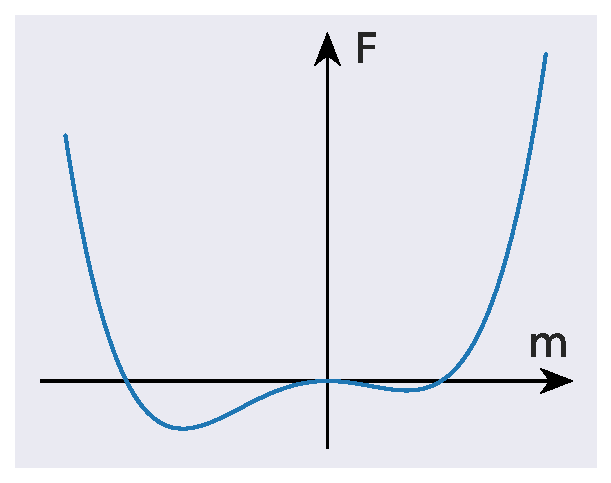
\includegraphics[width=\columnwidth]{figures/introduction/firstOrder-left-state.pdf}
	\end{subfigure}%
	\begin{subfigure}{0.33\textwidth}
		\centering
		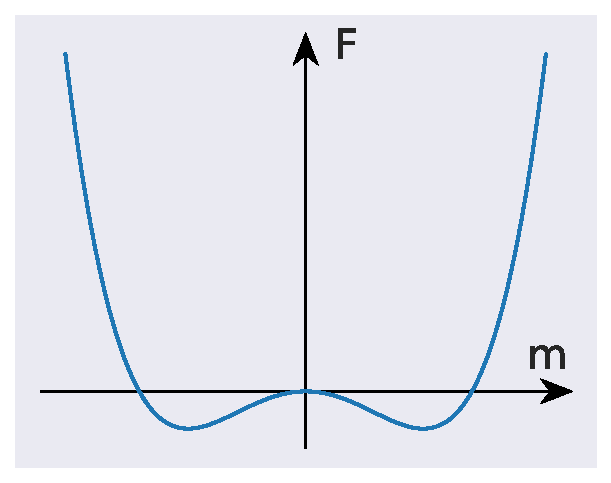
\includegraphics[width=\columnwidth]{figures/introduction/firstOrder-center-state.pdf}
	\end{subfigure}%
	\begin{subfigure}{0.33\textwidth}
		\centering
		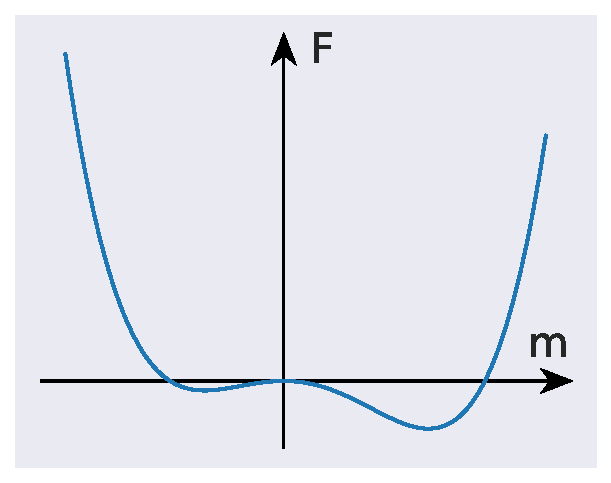
\includegraphics[width=\columnwidth]{figures/introduction/firstOrder-right-state.pdf}
	\end{subfigure}
	\caption{Curves of free energy in case of a first-order phase transition. Again we have three solutions, but only one is the true ground state and has lower energy than the other. A state with higher energy is a meta-stable state. Curves change shape as we change the sign of $\alpha(T)$ and $\gamma(T)$, corresponding to a phase order transition.}
	\label{gr:firstOrderLandau}
\end{figure}
\par
The toy model presented here can be solved exactly using the mean-field technique. Nevertheless, the question remains: How to compute the free energy for more complicated systems where a direct analytical approach does not work? One solution is to do it numerically or more precisely using the statistical techniques of Monte Carlo simulations that we will explore in the next chapter.  

\newpage
\section{Monte Carlo techniques}
The Monte Carlo methods are probably one of our most important numerical methods. The main idea is to obtain the approximate value of an integral by randomly sampling the value of the integrand at the expense of introducing statistical errors. Traditional grid methods that subdivide total volume become increasingly computationally expensive as we try to evaluate integrals in higher dimensions. For large systems, the number of configurations $i$ used in Eq.(\ref{eq:averageenergy}) is the integral of primary interest to physicists. The expectation value of some quantity $\expval{\xi}$, like the total energy of a system or a magnetization, is computed by summing over all possible states weighted by their respective probabilities.
\begin{equation}
	\expval{\xi} = \frac{\sum_\alpha \xi_\alpha e^{-\beta E_\alpha}}{\sum_\alpha e^{-\beta E_\alpha}} \mathcomma
\end{equation}
where $\beta = 1/kT$ and $E_i$ energy of a state. Sums like these are only feasible for small systems and generally cannot be computed exactly. One possible solution that we can take is to evaluate this sum only on a small appropriate subset of states and use this as an estimate. Suppose we take L states $\{ \alpha_1, \dots, \alpha_L\}$, then our estimate will be given by:
\begin{equation}
	\xi_L = \frac{\sum_{i=1}^{L}\xi_{\alpha_i}p_{\alpha_i}^{-1}e^{-\beta E_{\alpha_i}}}{\sum_{j=1}^L p_{\alpha_j}^{-1}e^{-\beta E_{\alpha_j}}} \mathperiod	
	\label{eq:estimator}
\end{equation}
We call $\xi_L$ the \textit{estimator} of $\xi$. It is clear from the procedure that as we take more samples, the estimator becomes more accurate, and in the limit $\lim_{L \rightarrow \infty} \xi_L = \expval{\xi}$. 
\par
The question then is how to choose $p_\alpha$. The most straightforward choice is to take all the states with an equal probability. Immediately we can see that for specific cases, this will be a terrible choice. Imagine evaluating an integral that is highly peaked around a particular value. Choosing points with equal probability will sample parts of the integral that do not contribute much toward the final result. Another way we can look at this from the physics point of view is when evaluating these sums at a very low temperature. Usually, only a handful of states will effectively contribute to the sum, so sampling over all (improbable) states will be a waste of computational time. The technique for selecting these most appropriate states is called \textit{importance sampling}. 
\par
Return to a physics example; we know that at a specific temperature, only the states in a small energy window will have measurable contributions to the sum, while an exponential factor will suppress the others. The natural choice for the probability distribution then presents itself; we will choose states according to their Boltzmann distribution. Looking at the equation Eq.(\ref{eq:estimator}), we can see that if we pick the states according to their Boltzmann weight $p_\alpha = Z^{-1} e^{-\beta E_\alpha}$, this expression simplifies considerably:
\begin{equation}
	\xi_L = \frac{1}{L} \sum_{i=1}^{L}\xi_{\alpha_i} \mathperiod
	\label{eq:mcestimation}
\end{equation}
We see that all the factors have canceled out. We are left with a simple sum, or more precisely, in order to get an estimate of a quantity $\xi$, we are going to sample states according to their Boltzmann distribution, measure $\xi$ in those states and then find an average over all of the measurements. When we settle on the desired distribution, the question remains how to realize it. One of the most widely used methods to achieve the desired distribution is through a \textit{Markov process}.
\par
In order to understand Markov processes, let us define a stochastic process at discrete times $t_1, t_2, t_3, \dots$ and a system with a finite set of states $\alpha_1, \alpha_2, \alpha_3, \dots$. Let us label with $X_t$ the state of a system at time $t$. The defining property of a Markov process is that:
\begin{equation}
	P(X_{t_n} = \alpha_{n} | X_{t_{n-1}} = \alpha_{n-1}, X_{t_{n-2}} = \alpha_{n-2}, \dots X_{t_{1}} = \alpha_{1}) = P(X_{t_n} = \alpha_{n} | X_{t_{n-1}} = \alpha_{n-1}) \mathcomma
\end{equation}
or in words, Markov process is \textit{memory-less}, the state of a system in the next time step only depends on the system's current state. Probability of generating state $\alpha_n$ given that system is in $\alpha_{n-1}$ is called \textit{transition probability} $P(\alpha_{n-1} \rightarrow \alpha_n)$. Another condition that these probabilities should satisfy is that they do not change over time. As with all probabilities, these should satisfy the fundamental requirement:
\begin{equation}
	\sum_{\alpha_n}P(\alpha_{n-1} \rightarrow \alpha_n) = 1 \mathcomma
	\label{eq:sumtoone}
\end{equation}
this means the process must generate some state, even the one the system already is in. We will end up with a \textit{Markov chain} of states by repeatedly generating new states. Suppose transition probabilities are chosen correctly after a sufficiently long time. In that case, the chain will come to an equilibrium, and its new states will satisfy the desired Boltzmann distribution.
\par
With chosen correctly, the following is meant. For the Markov process to achieve the desired equilibrium distribution, we must satisfy two additional conditions, \textit{ergodicity} and \textit{detailed balance}. Ergodicity, as we stated before, means that the Markov process should be able to reach any valid state from any valid state of the system if we let it run long enough. We know that every state in the Boltzmann distribution has a non-zero probability of appearing, so if this condition is violated, that would mean that there would be a pair of states $\alpha$ and $\gamma$ such that if we start from a state $\alpha$ we would never be able to reach state $\gamma$ and our goal of reaching the Boltzmann distribution would not be achievable. This does not mean that all transition probabilities should be non-zero, just that there should always be a path from two states that the process can follow.
\par
The second condition that we need to satisfy is the one of a detailed balance. This condition ensures that the final distribution we have reached is the desired Boltzmann distribution. What this exactly means is that the process has reached an equilibrium state. Let us take not a single state $\alpha$, but an ensemble with distribution $p_\alpha$. Then this ensemble is in equilibrium if the rate of states transforming into any state $\alpha$ is the same as the rate of states transforming from $\alpha$:
\begin{equation}
	\sum_{\beta}p_{\alpha} P(\alpha \rightarrow \beta) = \sum_{\beta}p_{\beta}P(\beta \rightarrow \alpha) \mathperiod
	\label{eq:balance}
\end{equation}
Then using Eq.(\ref{eq:sumtoone}) we get:
\begin{equation}
	p_{\alpha} = \sum_{\beta} p_{\beta}P(\beta \rightarrow \alpha) \mathperiod
\end{equation}
If our transition probabilities satisfy this condition, the probability distribution $p_{\alpha}$ will be the equilibrium distribution. Only imposing the condition in Eq.(\ref{eq:balance}) is not enough to guarantee that the probability distribution generated from any state will eventually settle to the desired distribution $p_\alpha$. In order to understand this, let us consider transition probabilities $P(\beta \rightarrow \alpha)$. We can form a large matrix where each entry in column $\alpha$ and row $\beta$ would be a transition probability from $\alpha$ to $\beta$; we call this a Markov matrix. If we label the probability that our system is in a state $\alpha$ at time $t$ with $p_{\alpha}(t)$, then we can say that a probability that the system is in state $\beta$ in a subsequent time step is:
\begin{equation*}
	p_{\beta}(t+1) = \sum_{\alpha} P(\alpha \rightarrow \beta) p_{\alpha}(t) \mathcomma
\end{equation*}
or in a more compact, matrix notation:
\begin{equation*}
	\bm{p}(t+1) = \bm{P} \cdot \bm{p}(t) \mathperiod
\end{equation*}
Now if we let this run for some time at the certain point the Markov chain will reach an equilibrium and we will have:
\begin{equation*}
	\bm{p}(\infty) = \bm{P} \cdot \bm{p}(\infty) \mathperiod
\end{equation*}
which is just a form of standard eigenvector equation. However, it is also possible for the Markov process to reach \textit{dynamic equilibrium}, which means that $\bm{p}$ rotates around several different values. Such rotation is called a \textit{limit cycle}. If this were the case, then the eigen equation would be:
\begin{equation*}
	\bm{p}(\infty) = \bm{P}^n \cdot \bm{p}(\infty) \mathcomma
\end{equation*}
where we call $n$ the length of the limit cycle. So how can we ensure limit cycles do not happen? The easiest way is to impose the condition of \textit{detailed balance}:
\begin{equation}
	p_{\alpha} P(\alpha \rightarrow \beta) = p_{\beta}P(\beta \rightarrow \alpha) \mathperiod
	\label{eq:detailedbalance}
\end{equation}
We can trivially see that if this condition is satisfied, then Eq.(\ref{eq:balance}) is also satisfied, but more importantly, we are eliminating the possibility of cycles. In order to understand why, look at the left side of Eq.(\ref{eq:detailedbalance}); this is an overall rate at which transition from $\alpha$ to $\beta$ happens, while the right side is the reverse. So this tells us that, on average, the system goes from $\alpha \rightarrow \beta$ as often as $\beta \rightarrow \alpha$. This would inherently be violated in the limit cycle as the states need to go from one to the other in a cyclic way. Another way we can justify the detailed balance condition is that most physical systems satisfy it in some way. The majority of the physical systems exhibit time-reversal symmetry. If we had a cycle in such a system upon reversing the arrow of time, the cycle would also reverse its direction. However, this reversal of cycle direction would completely change the system's dynamics, and any already established equilibrium would not be the same. In order to represent physical systems without this behavior, we would also like to remove it from our models.  
\par
We have established how to generate the desired probability, and from the detailed balance, our transition probabilities should satisfy the following:
\begin{equation}
	\frac{P(\alpha \rightarrow \beta)}{P(\beta \rightarrow \alpha)} = \frac{p_\beta}{p_\alpha} = e^{-\beta(E_\beta - E_\alpha)} \mathperiod
	\label{eq:acptprobratio}
\end{equation}
Here in the last step, we substituted the Boltzmann distribution. If we choose transition probabilities that satisfy this and the ergodicity condition, our Markov process should converge to the Boltzmann distribution. The procedure described so far looks straightforward; we need to choose the correct transition probability $P(\alpha \rightarrow \beta)$, and we are set. This is not always such an easy task, and there can be many different ways of creating a state $\beta$ from $\alpha$ that still, in the end, does not produce the desired distribution. There is a trick that can help us construct the desired process using any algorithm that we come up with, called the \textit{acceptance ratio}.
\par
The main observation that lies at the heart of the acceptance ratio is that we can modify the probability of a state staying at the same state as much as we want (still with the constraint that probability should be positive and less than one) and automatically satisfy Eq.(\ref{eq:acptprobratio}). This allows us to tune our transition probabilities as we like and then, by adjusting the ``staying'' probability, satisfy the required condition. Let us see how we can do this. First, we will break the transition probability into two parts:
\begin{equation*}
	P(\alpha \rightarrow \beta) = g(\alpha \rightarrow \beta) A(\alpha \rightarrow \beta) \mathperiod
\end{equation*}
The first quantity on the right side, $g(\alpha \rightarrow \beta)$, is called the \textit{selection probability}, the probability given an initial state $\alpha$ that we will end up in the state $\beta$. The second quantity, $A(\alpha \rightarrow \beta)$, is the acceptance ratio, the probability that we accept the generated state. Now if we expand the Eq.(\ref{eq:acptprobratio}) in terms of selection probability and acceptance ratio, we will get:
\begin{equation}
	\frac{P(\alpha \rightarrow \beta)}{P(\beta \rightarrow \alpha)} = \frac{g(\alpha \rightarrow \beta) A(\alpha \rightarrow \beta)}{g(\beta \rightarrow \alpha) A(\beta \rightarrow \alpha)} \mathperiod
	\label{eq:selecprobAcceptratio}
\end{equation}
From the equation above, we see that the ratio $\frac{A(\alpha \rightarrow \beta)}{A(\beta \rightarrow \alpha)}$ can take any value between $0$ and $\infty$. This means that selection probabilities can be tuned to anything we like, and the acceptance ratio will absorb any difference. Partitioning transition probabilities into acceptance ratio and selection probability enables us to create a Monte Carlo algorithm that will generate random state $\nu$ given state $\mu$ and then adjust selection probabilities for these states so they satisfy the condition in Eq.(\ref{eq:selecprobAcceptratio}) and reach the desired Boltzmann distribution. So we finally reached a theoretically complete algorithm to generate the desired Boltzmann distribution. 
\begin{algorithm}[H]
	\caption{Markov process algorithm}
	\begin{algorithmic}[1]
		\State design an algorithm that will generate a random new state $\beta$ given that we are at $\alpha$ with some probabilities $g(\alpha \rightarrow \beta)$
		\State accept that state with the probability $A(\alpha \rightarrow \beta)$ 
		\State adjust acceptance ratios in such a way that we satisfy Eq.(\ref{eq:selecprobAcceptratio})
		\State after reaching it's equilibrium state, Markov process will have the desired Boltzmann probability distribution.
	\end{algorithmic}
	\label{algo:Markovchain}
\end{algorithm}
\par
The algorithm outlined above looks nice and easy, but we still need to pay attention to how we choose our acceptance ratios. If they are small, we will usually stay in the same state and not move at all. We need to make a delicate balance so that our algorithm explores the phase space without slowly crawling around it. This can be ensured by making the acceptance ratio close to one. The good thing is that Eq.(\ref{eq:selecprobAcceptratio}) only fixes ratio $\frac{A(\alpha \rightarrow \beta)}{A(\beta \rightarrow \alpha)}$, which means that we have the freedom to multiply both of them with some constant. In practice, this often means we fix the larger to one and then multiply the other with an appropriate constant to keep the ratio fixed. Another thing that we can try to do while designing a new algorithm is to put as much of $P(\alpha \rightarrow \beta)$ into the selection probability because the perfect algorithm would be the one where the states are only selected by the transition probability, which means acceptance ratio is always one. In the absence of a perfect, we can try to keep our acceptance ratio as close to one as possible.
\par
We have covered the theoretical part of designing an algorithm to ensure that the resulting chain will have the Boltzmann distribution. Let us look into one of the most common algorithms, \textit{Metropolis algorithm}.
\par
In order to show all the details of how this algorithm works, we will again use the Ising model, where ``spins'' $s_i$ live on the sites of a lattice and can take values $\{ -1, +1\}$. If we have $d$ dimensional lattice of size $N$, our system can be in $2^{N^d}$ possible states. These numbers grow exponentially as we go to higher dimensions and bigger lattices. This type of problem is the perfect playground for Monte Carlo methods. To recall from Eq.(\ref{eq:classicIsing}) the Ising Hamiltonian is:
\begin{equation}
	E = -J \sum_{\langle i j \rangle} s_i s_j - h \sum_i s_i \mathcomma
	\label{eq:classicIsing2}
\end{equation}
where $J$ is the interaction energy between the nearest neighbors and $h$ is the external magnetic field. The most common questions regard the values of magnetization $m$ and specific heat $C_V$ at the fixed temperature, which we computed earlier in the mean-field limit. For simplicity, we will consider the Ising model with no external magnetic field $h=0$
\par
As we showed in the section \ref{sec:statPhys} in the thermal equilibrium, energies of the system stay in a tiny window around the mean value; they do not fluctuate much. We want to replicate this behavior in our algorithm as well. The easiest way we can do this is by flipping a single spin at a time. This type of algorithm has a \textit{single spin-flip dynamics}. In the $d$ dimensional lattice, the maximum energy difference would be $2zJ$, where $z$ is \textit{lattice coordination number}, or simply the number of neighbors a site has. Another advantage of flipping a single spin is that we also satisfy the ergodicity condition.
\par
The Metropolis algorithm now sets the selection probabilities $g(\alpha \rightarrow \beta)$ equal for all possible states $\beta$ while setting it to zero for all the other ones. Let us say that we have $N^d$ spins in our system; that means there are $N^d$ different spins that we could flip and also $N^d$ different states that we could end up in. This means that we have $N^d$ different selection probabilities $g(\alpha \rightarrow \beta)$ that are non-zero, and all of them have the same value:
\begin{equation*}
	g(\alpha \rightarrow \beta) = \frac{1}{N^d} \mathperiod
\end{equation*}
In practice, we randomly pick a site with equal probability and flip its spin. Now our condition of the detailed balance (\ref{eq:selecprobAcceptratio}) is:
\begin{equation}
	\frac{P(\alpha \rightarrow \beta)}{P(\beta \rightarrow \alpha)} = \frac{g(\alpha \rightarrow \beta) A(\alpha \rightarrow \beta)}{g(\beta \rightarrow \alpha) A(\beta \rightarrow \alpha)} = \frac{A(\alpha \rightarrow \beta)}{A(\beta \rightarrow \alpha)} = e^{-\beta (E_\beta - E_\alpha)} \mathperiod
	\label{eq:metropolisBalance}
\end{equation}
If we remember the algorithm design steps, we will set the largest of the acceptance ratios to $1$ and adjust the other one to make this the most efficient algorithm. Assume that state $\alpha$ has the lower energy than $\beta$, $E_\alpha \le E_\beta$. Then the larger acceptance ratio would be where we go from the state $\beta$ to the state $\alpha$, $A(\beta \rightarrow \alpha)$, we will set it to $1$. In order to satisfy Eq.(\ref{eq:metropolisBalance}) we must then set $A(\alpha \rightarrow \beta) = e^{-\beta (E_\beta - E_\alpha)}$. Now our final algorithm is:
\begin{equation}
	A(\alpha \rightarrow \beta) = \begin{cases}
		e^{-\beta (E_\beta - E_\alpha)} & \text{if } E_\beta - E_\alpha \ge 0 \\
		1 & \text{otherwise}
	\end{cases} \mathperiod
\end{equation}
Put in words, this means that if we select a state with lower energy, we always accept the move, and if we select the state with higher energy, we will accept it with the probability $e^{-\beta (E_\beta - E_\alpha)}$.
\par
So far, we only said that we must wait long before our system reaches equilibrium. Now we will specify what this exactly means. First, let us define this period. The time we need to wait for the system to reach the thermal equilibrium is called the \textit{thermalization time}, $\tau_T$. How do we know how long is enough? We could look at the state of a system as in the Fig.(\ref{gr:configurations}) and then gauge when it has reached the equilibrium, but the better and simpler way to do this is to plot some quantity, like energy or magnetization, over "time" and see when it settles around the average value. The usual way to measure time in Monte Carlo simulations is in terms of \textit{sweeps}. Sweep is the number of updates we do to flip all the spins on the lattice. So if we sequentially try to flip spins in the lattice after $N^d$ attempts, we will complete one sweep. In Fig.(\ref{gr:themalization}), we see that after $300$ sweeps, the average magnetization and energy have thermalized. However, in practice, this is not always enough. Sometimes if the energy landscape is particularly rough, we could end up in one of the \textit{local minima} and oscillate around it. In order to avoid this, we can start our simulation with different initial conditions, like at $T=0$ (all spins aligned) and $T=\infty$ (completely randomly oriented spins), and let them run. When two runs settle around the same average value, we have good reason to believe that thermalization has completed and we have reached equilibrium Fig.(\ref{gr:themalizationTwoRuns}). If we are still worried that we might have ended up in some local minimum, we can do a third run with a different randomly oriented configuration and repeat the same procedure.
\begin{figure}[H]
	\centering
	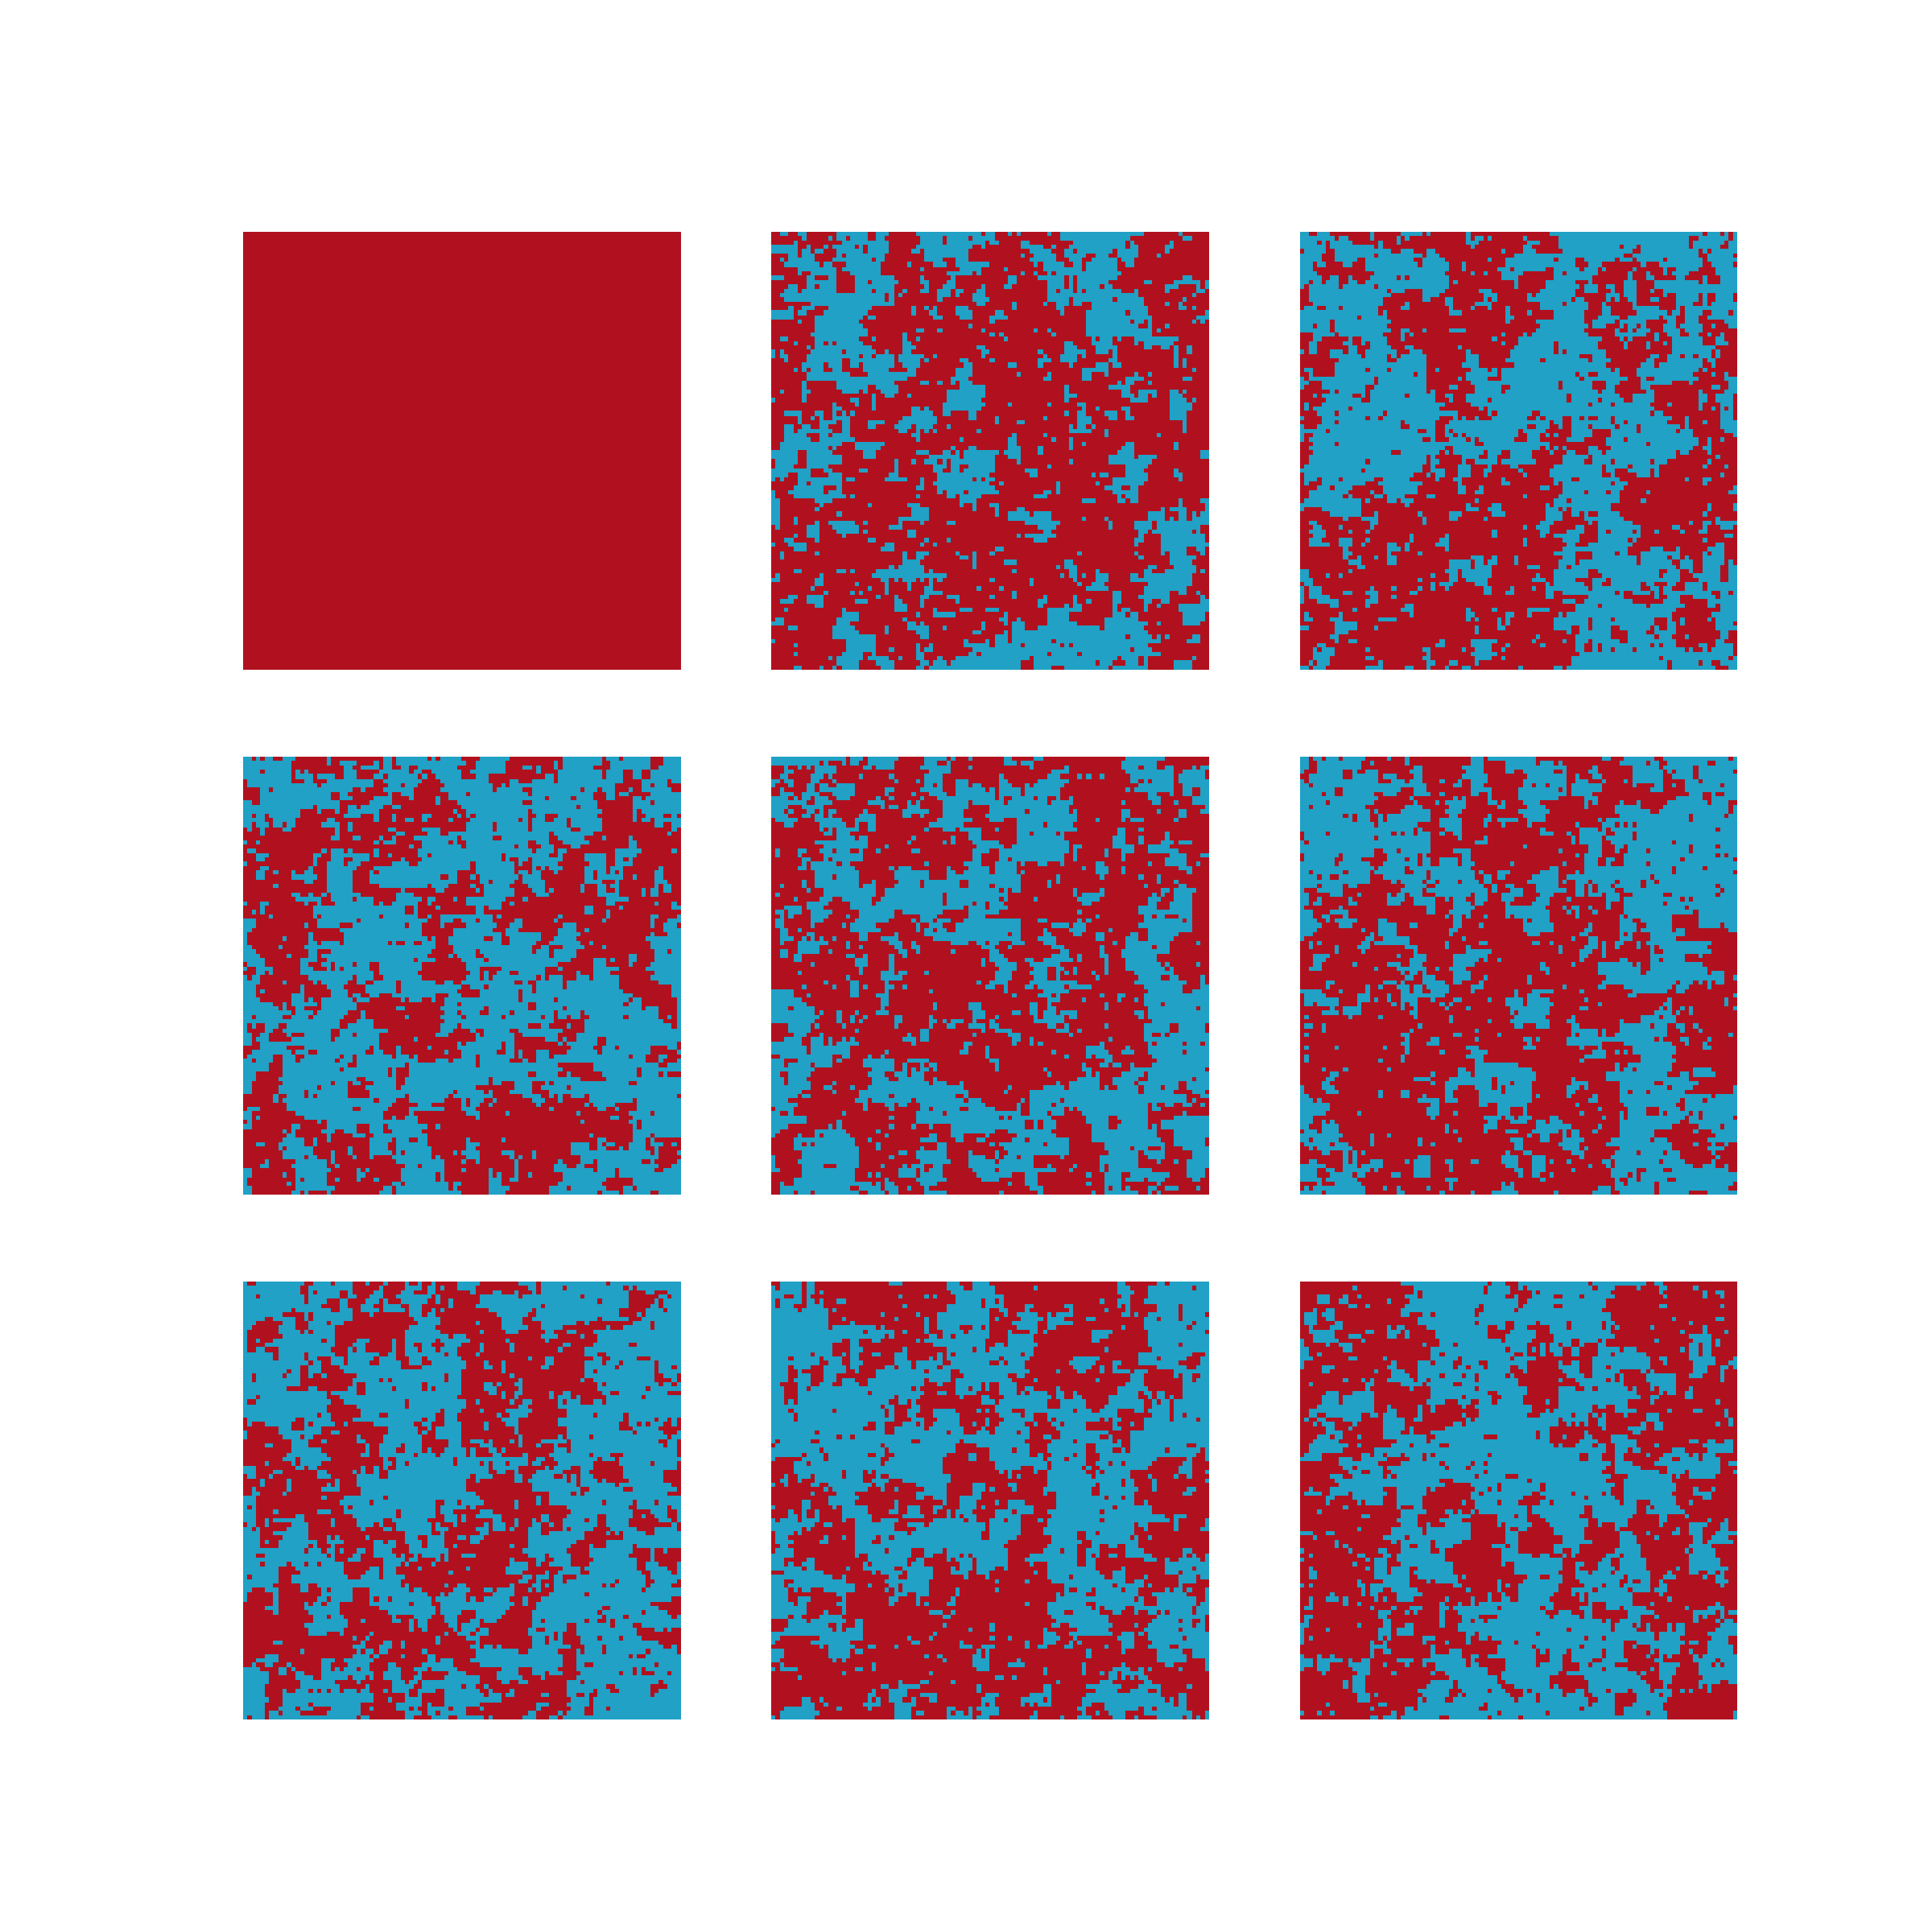
\includegraphics[width=13cm]{figures/introduction/configurations.pdf}
	\caption{Time slices of the spin configuration on a $100 \cross 100$ lattice throughout the simulation. Red are spins $-1$, and blue spins are $+1$. We have started at $T=0$ configuration with all the spins aligned and then simulated $J=1$ and $T=2.4$ for 1000 sweeps. Slices were taken every 100 sweeps. The graph shows that the system reached equilibrium configuration around the 400th sweep.}
	\label{gr:configurations}
\end{figure}
\begin{figure}[H]
	\centering
	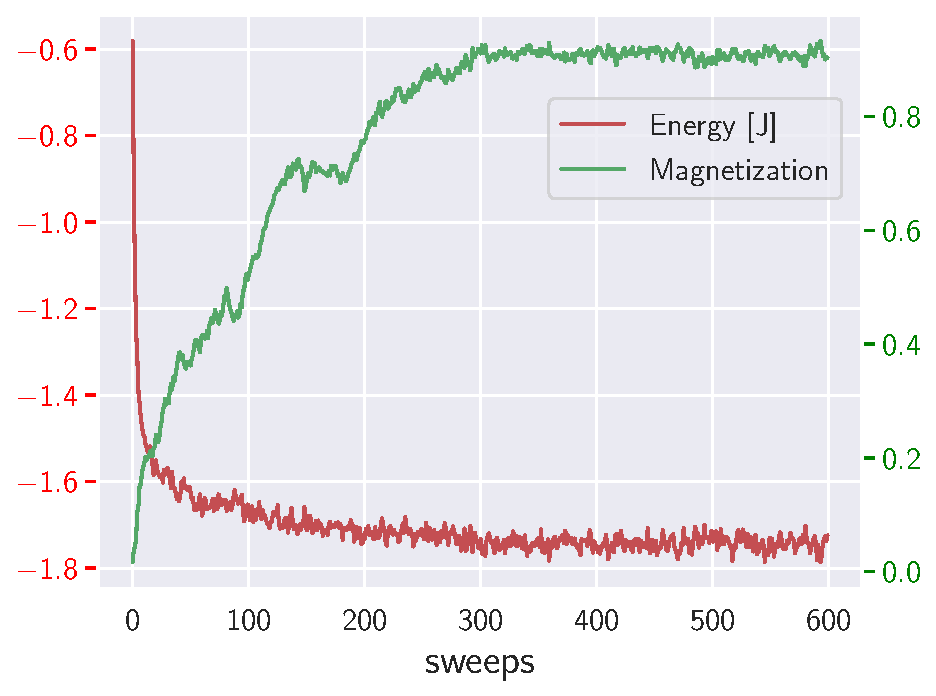
\includegraphics[width=7cm]{figures/introduction/thermalization.pdf}
	\caption{Graph of magnetization per site (green squares) and energy per site (red circles) for a 2D Ising model with no external magnetic field ($h=0$) on a lattice $N=100$, $J=1$ near the critical temperature ($T_c \sim 2.26$)  $T=2.0$. We can see that energy and magnetization reach their thermal values around 300-400 sweeps.}
	\label{gr:themalization}
\end{figure}
\begin{figure}[H]
	\centering
	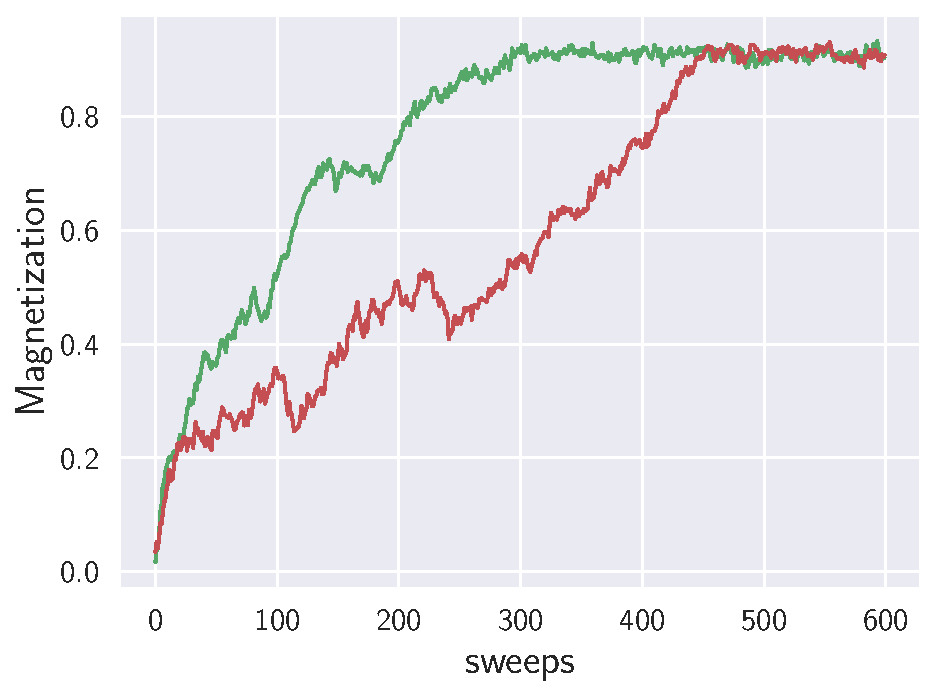
\includegraphics[width=7cm]{figures/introduction/thermalizationTwoStarts.pdf}
	\caption{Graph of magnetization per site for two 2D Ising models with different initial configurations (at $T=\infty$), no external magnetic field ($h=0$) on a lattice $N=100$, $J=1$ and equilibrium temperature $T=2.0$. We can see that two different initial configurations had different paths through the phase space, but both have settled on the same value for the magnetization per site. Waiting for around 500 sweeps would guarantee that our Monte Carlo chain has thermalized for these values of $J$ and $T$.}
	\label{gr:themalizationTwoRuns}
\end{figure}
\par
We have established how to get an adequately converged Monte Carlo simulation. The next step is measuring some quantity, such as energy or magnetization. If we recall our algorithm's exact dynamics, we will realize that the single flip dynamics states are actually highly correlated. This implies that two or more successive measurements will be correlated. In order to solve this, we will wait for a certain amount of sweeps between successive measurements, called \textit{correlation time}, $\tau$.
\par
In order to estimate autocorrelation time, we will use \textit{time-displaced autocorrelation function}. We give here an example of it for magnetization:
\begin{equation}
	\chi(t) = \int \dd t^\prime (m(t^\prime)m(t^\prime + t) - \expval{m}^2) \mathperiod
	\label{eq:autocorrfunc}
\end{equation}
This is just the two-point function we have seen in the first part of the introduction, but now instead of being between two sites $i$ and $j$, it is between two time-steps $t$ and $t^\prime$. One assumption that we have to make in order to make this work is that the autocorrelation function falls off exponentially at long times (which is a very reasonable assumption to make):
\begin{equation}
	\chi(t) = e^{-\frac{t}{\tau}} \mathperiod
	\label{eq:expautocorrtime}
\end{equation}
We can see from this that waiting time $\tau$ between two measurements will only reduce the autocorrelation function by $1/e$, so the most common practice is to take measurements every $2\tau$ sweeps. Given the exponential form of the autocorrelation function Eq.(\ref{eq:expautocorrtime}) we can define what the \textit{integrated correlation time}:
\begin{equation}
	\int_{0}^{\infty} \frac{\chi(t)}{\chi(0)} \dd t = \int_{0}^{\infty} e^{-\frac{t}{\tau}} \dd t = \tau \mathperiod
\end{equation}
This equation gives us a direct way of estimating the autocorrelation time. To complete the procedure, we need a discrete version of the Eq.(\ref{eq:autocorrfunc}) that we can use in order to estimate the autocorrelation time:
\begin{equation}
	\chi(t) = \frac{1}{t_{\text{max}} - t} \sum_{t^\prime = 0}^{t_{\text{max}} - t}m(t^\prime)m(t^\prime + t) - \left ( \frac{1}{t_{\text{max}} - t} \right )^2 \sum_{t^\prime = 0}^{t_{\text{max}} - t} m(t^\prime) \sum_{t'' = 0}^{t_{\text{max}} - t} m(t'' + t) \mathperiod
\end{equation}
When using this equation to calculate $\chi$, we have to take care that at long times when $t$ gets close to $t_{\text{max}}$, the upper limit in the sums gets very small, and because of the statistical nature of the measurements, errors can get very large. In order to avoid this, we can run a simulation long enough (hopefully for several autocorrelation times), and then we would not need to worry about the long tails of $\chi(t)$.
\par
We have established how to generate new states from the old one, measure quantities of interest and calculate autocorrelation time so our sample end up uncorrelated. The final step is to quantify the errors of those measurements in order to get the complete results. Our errors can be divided into two categories, \textit{systematic errors} and \textit{statistical errors}. We have introduced systematic errors due to the procedures we used to measure observables. Another source of systematic errors can be if we do not wait long enough for the system to thermalize. Also, if we do not collect enough samples after the thermalization and let our samples be correlated. Systematic errors are hard to measure, and we can mitigate them by following the correct procedure for reaching the equilibrium and collecting enough uncorrelated samples after. On the other hand, statistical errors are more easily measured; they arise from the random nature of the Monte Carlo simulations and the system's thermal fluctuations. The simplest way to minimize statistical errors is to collect more uncorrelated samples.
\par
Statistical errors of a quantity are relatively easy to estimate. As we stated, due to the thermal fluctuations from one state to the other, measurements (let us take magnetization $m$) vary around some average value. The natural way is to take the mean of all of these samples as the actual average value and the error of the mean as an error to that estimate. Let us take $N$ measurements of magnetization $m$; our best estimator for the true average is the mean value:
\begin{equation}
	\expval{m} = \frac{1}{N} \sum_{i=0}^N m_i \mathcomma
\end{equation}
and the estimate of the standard deviation of the mean is:
\begin{equation}
	\sigma^2 = \frac{1}{N(N-1)}\sum_{i=0}^N (m_i - \expval{m})^2 = \frac{1}{N-1} \left ( \expval{m^2} - \expval{m}^2 \right ) \mathperiod
	\label{eq:stdest}
\end{equation}
This might look similar to the susceptibility we defined in section \ref{sec:statPhys}. There we calculated susceptibility as a variance of the energy over the given ensemble of states, while here, the $\sigma^2$ is an unbiased estimator for the true variance of the mean. An essential fact about Eq.(\ref{eq:stdest}) is that it assumes that our samples are statistically independent. If, on the other hand, we have samples that were sampled every $\Delta t$ sweeps and the autocorrelation time is $\tau$, then our estimate for the standard deviation is\cite{newman1999monte}:
\begin{equation}
	\sigma^2 = \frac{1 + \frac{2\tau}{\Delta t}}{N-1}\left (\expval{m^2}-\expval{m}^2 \right) \mathperiod
\end{equation}
We can immediately see that if $\Delta t \gg \tau$, this expression would reduce to the Eq.(\ref{eq:stdest}), but often, because of practical reasons, we have $\Delta t \ll \tau$. If that is the case, then we can practically ignore the $1$ and note that the number of samples is the total amount of time divided by the sampling interval:
\begin{equation*}
	N = \frac{t_{\text{max}}}{\Delta t} \mathperiod
\end{equation*}
For the large number of samples we have:
\begin{equation}
	\sigma^2 = \frac{2\tau}{t_{\text{max}}}\left(\expval{m^2}-\expval{m}^2 \right) \mathperiod
\end{equation}
A neat property of this estimation is that our standard deviation does not depend on $\Delta t$, which means we can sample with any frequency we want.
\par
In some cases, it is not feasible to calculate the errors this way, for example, in any derived quantities that depend on the average values, like specific heat. We only have access to the average values after we finish running and do not have access to specific heat during every time step. In principle, we could do a detailed analysis of error propagation taking into account how $\expval{E}$ and $\expval{E^2}$ errors are correlated, but this would be a complex and error-prone process, also the resulting equation would be highly dependent on the initial equation we used to calculate the observable. This would mean that every time we have a different form of an equation, we would have to do the same analysis again. Luckily, we can use robust methods to estimate an error of these quantities. The most known and well-established is \textit{bootstrap method}.
\par
Bootstrap belongs to a class of the \textit{resampling methods}. Let us first sample $N$ measurements of the energy. Next, we can consider these $N$ measurements as a state space for the energy, forming some probability distribution. In essence, we want to infer the information about this probability and functions of it. For energy, our goal would be to calculate the mean and the error. The idea is to draw $N$ new samples with equal probability and repetition from the original set of $N$ samples, repeating the procedure $M$ times. Calculating the mean for each set of $M$ repetitions would get us $M$ values of the mean. These new $M$ values represent the probability distribution of the mean, and we can use them to calculate the standard deviation. This method is advantageous when, for example, we have stored some observable values but want to estimate some function of it. 
\par
An example of a function of an observable would be the specific heat $C_V(\expval{E}, \expval{E^2})$. The procedure would go like this, from initial $N$ measurements sample new $N$ samples with repetition $M$ times. For each of the $M$ samples, we compute $C_V$, leaving us with a list of specific heats that we call $a$. Now it turns out that the standard deviation of the specific heat is given by\cite{newman1999monte}:
\begin{equation}
	\sigma^2 = \langle a^2 \rangle - \langle a \rangle^2 \mathperiod
\end{equation}
This means we take the standard deviation of the newly constructed list of $C_V$ values, and the mean would simply be the average of $a$. It can also be shown that even if we draw correlated samples, bootstrap will estimate standard deviation equally well. 
\par
So far, we have covered the basic steps and algorithms for constructing the Markov process with the desired distribution. These steps are the same for multiple fields where Monte Carlo simulation might be used. Now we focus on the applications in physics. We will stick with the $2D$ Ising model. At the mean-field level, Ising in $2D$ dimensions goes through the phase transition as we change the temperature. We can think of it this way, at a very high temperature $T=\infty$, all the spins are randomly oriented, with plenty of energy at their disposal and no order among the spins. This is a paramagnetic phase, where the total magnetization of the system is zero.
\par
As we decrease the energy, spins try to align more and more, as this is now energetically more favorable, and at a certain point, the total magnetization becomes finite. This phase, where the total system has non-zero magnetization, is the ferromagnetic phase. As discussed in the previous section, this phase transition belongs to the second-order phase transitions class. Second order means the second derivative of the free energy is discontinuous. The standard second derivative is specific heat $C_V = -T \left(\pdv[2]{F}{T}\right)\bigg\rvert_{V=\text{const}}$. The straightforward way to see if the system goes through a phase transition is to plot specific heat as a function of the changing variable. Thus, specific heat should be diverging at the transition point for the second-order phase transition. Strictly speaking, diverging behavior is only seen in the thermodynamic limit (for infinite systems). Since we can only simulate systems of finite sizes, we will see that specific heat will develop a sharper peak as we increase the size. This can be seen in Fig.(\ref{gr:Ising2DCv}). We can compare the value of $T$ with the exact known critical temperature $T_c = \frac{2J}{\ln(1 + \sqrt{2})} \approx 2.27J$, as well as the meanfield result $T_c = 4J$.
\begin{figure}[H]
	\centering
	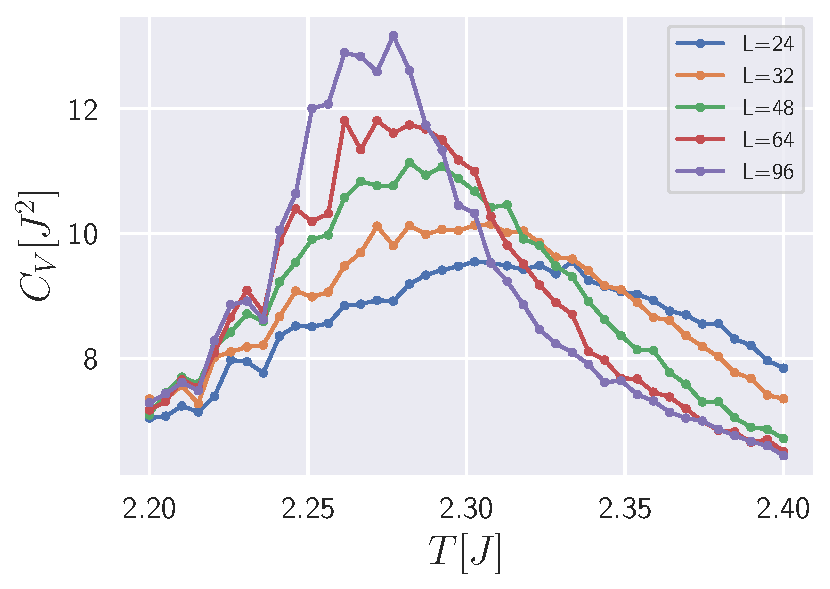
\includegraphics[width=7cm]{figures/introduction/Ising2DCv.pdf}
	\caption{Specific heat curves $C_V$ of 2D Ising for $J=1$ on a square $L \cross L$ lattice around the transition point for different system sizes. Strictly speaking, specific heat only shows diverging behavior for infinite system sizes. Because of this, determining the exact point of transition through these curves is not very precise. The exact value of critical temperature is $T_c=\approx 2.27$, while the mean-field result is $T_c = 4$ (way off on the above graph).}
	\label{gr:Ising2DCv}
\end{figure}
\par
Now that we have identified the existence of a continuous phase transition, we would like to describe it in more detail for two reasons: both related to the numerical implementations. The first is critical slowing down, and the second is finite size determination of free phase transition. Landau's theory of phase transitions shows that the free energy has a singularity in the thermodynamic limit, usually described by a power law of the observables near the critical point. Underlying this divergence is a divergent \textit{correlation length} $\xi$. It gives a sense of how correlated or ordered the spins in our system are, and it is diverging near the transition according to the:
\begin{equation}
	\xi \sim |T - T_c|^{-\nu} \mathcomma
\end{equation}
whit $\nu$ the \textit{critical exponent}. The specific heat has a similar shape near the criticality:
\begin{equation}
	C_V \sim |T-T_c|^{-\alpha} \mathcomma
\end{equation}
with the difference that $\alpha$ can now be positive and negative. From the renormalization group theory, we know that these critical exponents are related by scaling relations. In most cases, only two exponents are independent, and the rest can be derived from them\cite{newman1999monte}. These two exponents fully characterize the critical behavior of the model. Also, it can be shown that models often have the same set of these critical exponents and can be further categorized in \textit{universality} classes. This means that models with different microscopic details exhibit the same behavior near the critical point, and details get washed away. Everything is controlled by $\nu$.
\par
The issue is that these divergences only occur in the thermodynamic limit. For finite-size systems, the critical behavior is smeared out, and estimating the location of the peak will introduce the error. Due to a related problem, critical slowing down, one cannot simply sample more\cite{newman1999monte}. 
\par
One better way to determine the transition point and critical exponents is through the technique of \textit{finite size scaling}. Using the results from the renormalization group, we know that the magnetization scale, close to the transition, with system size $L$ as:
\begin{equation}
	\expval{m_L} \sim L^{\frac{\beta}{\nu}}\tilde{M}\left[L^{\frac{1}{\nu}}(T-T_c)\right] \mathcomma
	\label{eq:magScaling}
\end{equation}
where $\tilde{M}(x)$ in unknown scaling function. We can see from the Eq.(\ref{eq:magScaling}) that $\expval{m_L}/L^{\beta / \nu}$ at $T=T_c$ will be independent of the system size, as the argument of $\tilde{M}$ will be zero. So this means that scaled magnetizations will all have the same value precisely at the critical temperature. On the plot where these different scaled magnetization curves would be drawn together at the point of critical temperature, they would intersect each other. If we want to be completely precise, we are ignoring some non-analytic corrections to the scaling so the curves intersect only at the same point in the sense $L\rightarrow\infty$. Doing finite-size scaling using this method is not helpful in practice because neither $\beta$ nor $\gamma$ is known a priori. A better approach is to compute a combined quantity that is dimensionless. One such quantity is the \textit{Binder cumulant}\cite{bindeCumulant}:
\begin{equation}
	U = \frac{1}{2} \left[3 - \frac{\expval{m^4}}{\expval{m^2}^2}\right] \sim \tilde{G}\left[L^{\frac{1}{\nu}}(T-T_c)\right] \mathperiod
\end{equation}
In the limit, $T\rightarrow 0$, Binder cumulant goes to $1$; in the opposite limit, when the temperature $T\rightarrow \infty$ Binder goes to $0$. Because Binder cumulant is a dimensionless quantity, different $L$ curves should approximately intersect at the same point, given that the non-analytic corrections are small. We can use this to determine $\nu$, see Fig.(\ref{gr:2DIsingBinder}). On the other hand, if we plot all the curves with the appropriate critical scaling $\nu$ on the plot $U$ vs. $L^{1/\nu}(T-T_c)$ they all fall on top of each other as in Fig.(\ref{gr:2DIsingBinderCollaps}).

\begin{figure}[H]
	\centering
	\begin{subfigure}[c]{0.5\textwidth}
		\centering
		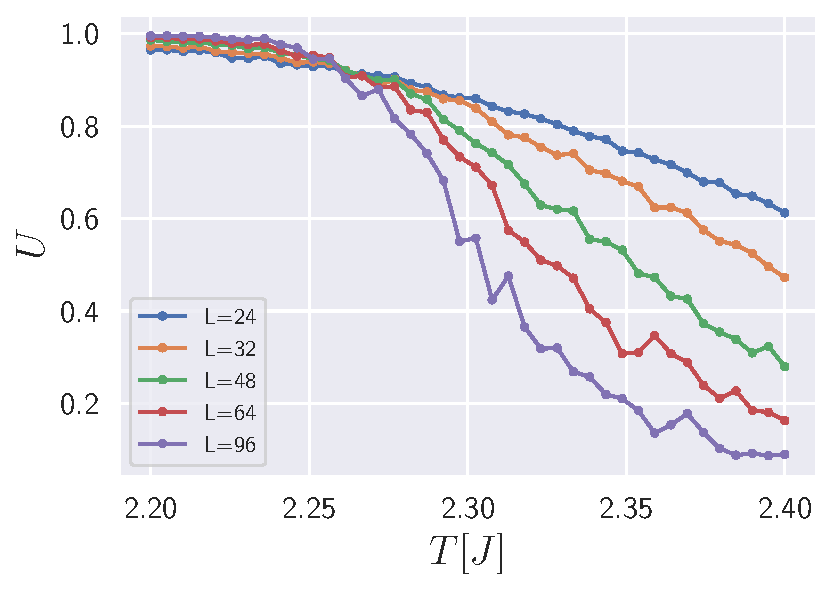
\includegraphics[width=\textwidth]{figures/introduction/Ising2DBinder.pdf}
		\caption{}
		\label{gr:2DIsingBinder}
	\end{subfigure}%
	\begin{subfigure}[c]{0.5\textwidth}
		\centering
		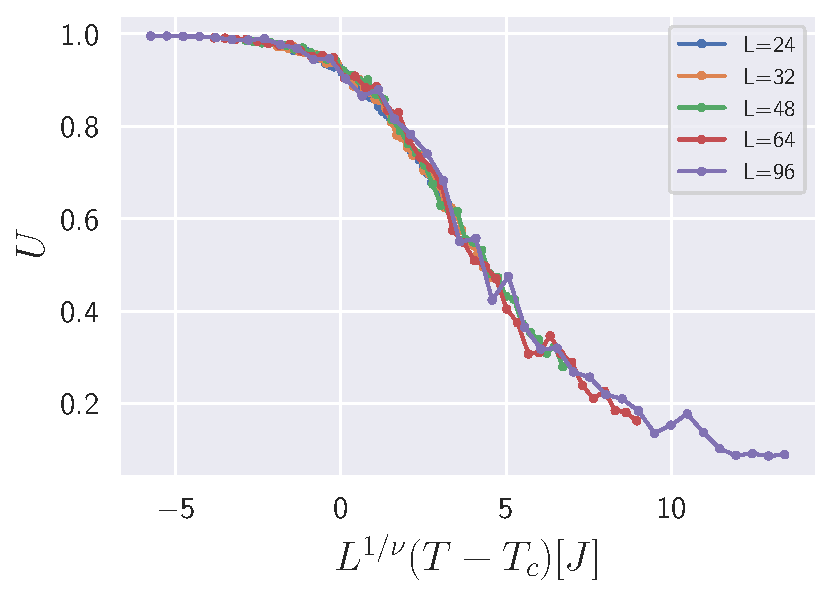
\includegraphics[width=\textwidth]{figures/introduction/Ising2DBinderCollapse.pdf}
		\caption{}
		\label{gr:2DIsingBinderCollaps}
	\end{subfigure}
	\caption{\textbf{(a)} Binder cumulant curves for different system sizes. Because the Binder cumulant is a dimensionless quantity, all the curves cross at the same point, given that the non-analytic corrections are small. This method is more robust and reliable for determining the exact critical temperature $T_c \sim 2.26$. \textbf{(b)} After doing the finite size scaling for the Binder cumulant data in Fig.(\ref{gr:2DIsingBinder}), all the curves have collapsed on a single line. We can use Binder cumulant curves to determine the exact position of $T_c$ and then use that to fit all the curves to determine the critical exponent $\nu=1$.}
\end{figure}
\par
In this thesis, we shall use the Binder cumulant differently to determine the order of a phase transition. In the case of continuous, second-order phase transition, the Binder cumulant has a smooth transition. In the case of a first-order phase transition, instead of being continuous, the Binder cumulant has a dip at the point of the critical transition. The dip occurs because, at the point of transition order, the parameter experiences a discontinuity which is also present in any functions that depend on it. This dip diverges with the system size\cite{bindeCumulant}. We can use Binder cumulant to see whether the actual phase order exists and determine its order. Another possibility is the case of a weak first-order transition, where the Binder cumulant still exhibits a dip, but this dip is not diverging with the system size.
\newpage
\section{Machine learning}
Since discovering quantum mechanics, physicists have sought better, more accurate approximation techniques to solve real-world quantum problems. As we know from the introductory quantum mechanics courses, only a handful of toy models Schr\"{o}dinger equation can be solved exactly. If we start considering systems with many interacting particles, our analytical methods can only serve up to a certain point. Some well-known numerical techniques, such as exact diagonalization and tensor networks, also start having problems when we apply them to systems of many highly interacting particles. The Monte Carlo techniques reviewed in the previous section can provide approximate answers. Recently, one of the pioneering methods that used machine learning was introduced by Carleo and Troyer \cite{carleoTroyer}, where they consider an RBM network as an ansatz in variational quantum Monte Carlo.
\par
The term \textit{machine learning} (ML) has become an everyday expression in recent times. It can be defined as a sub-field of Artificial intelligence primarily tasked with developing algorithms for learning from experience (or data). The backbone of ML is based on applied statistics while also drawing some ideas from statistical physics. The main goal of ML is to estimate unknown, often very complicated, functions that depend on a large number of unknowns and give useful predictions on new (unknown) data. This program of pushing ever bigger and more complex algorithms led to the development of \textit{deep learning} (DL), where massive networks with millions of parameters are trained on more extensive data sets. The development of highly efficient and parallel GPUs led to a boom in developing new ML and DL algorithms. The main appeal of ML and DL is that some tasks, hard to put in an algorithmic form, can now be tackled with ease. A typical example would be recognizing a cat, dog, or human being in a picture or detecting a new phase state of a quantum matter. ML and DL have grown tremendously in recent years; hence a complete introduction is simply impossible here, and we will try to introduce the essential elements of both fields used in the later chapters.
\par 
Before actually doing any computation, we need to establish the main ingredients we need to make the computer learn \cite{MLintro}:
\begin{itemize}
	\item a \textit{task} that we need to solve, like regression, classification, generating pictures, or learning how to play a game
	\item \textit{data} in the case of ML and DL, we can look at the data as an experience that our algorithm lives and learns from. Some forms of data can be given in a table, like pictures of handwritten digits and their labels, or it can be given in the form of a reward, for example, how long the robot managed to walk
	\item a \textit{model} that learns from the data.
\end{itemize}
Usually, more than these are needed to specify the learning algorithm fully. We need to define a measure that will compare the performance of our algorithm with the actual known data. Our task is to minimize this difference between the predicted and known data.
\par
\begin{itemize}
	\item \textit{Regression} can be viewed as one of the most common forms of ML. We assume that there is some (potentially unknown) relation between two variables $\vb{x}$ and $\vb{y}$, and we try to learn what that relation is. We will call variable $\vb{x}$ an input and variable $\vb{y}$ an output. These variables are not restricted to a single dimension; they are often multi-dimensional. As stated, our task is to find some function $f$ that will satisfy the relation $\vb{y}=f(\vb{x})$. The simplest example would be a linear regression, where we assume that our function has the form $\vb{y}=\vb{A}\vb{x} + \vb{b}$, and we have free parameters $\vb{A}$ and $\vb{b}$ to optimize.
	\item \textit{Classification} is a task where our output variables do not have a continuous output but are rather discrete and categorized in different \textit{classes (labels)}. In comparison with the regression, we are now trying to find a function that will map our input $\vb{x}$ to a target $\vb{y}$ but also encode a representation for multiple different classes. The simplest example would be a binary classification, a case when we need to distinguish between two different labels, for example, is this a picture of a cat or not. One of the most famous datasets that we will use later is MNIST (Modified National Institute of Standards and Technology), which consists of $70.000$ handwritten digits distributed over $10$ ``classes'', the digits $0, 1, 2, \dots, 9$. 
\end{itemize}
\par
The data, the main ingredient in many machine learning tasks, comes in datasets $\mathcal{D}$, containing data points $\vb{x}_i$, $\mathcal{D} = \{\vb{x}_i\}$. Depending on the information available in our data set, we can divide the types of learning we can do:
\begin{itemize}
	\item \textit{Supervised learning} is a class of problems where our data points are \textit{labeled}. It can either be a regression or a classification. Methods used to do supervised learning can be classical ML or more modern and complex DL. 
	\item \textit{Unsupervised learning} is applied when data does not have accompanying labels that we can use. Some examples of unsupervised learning methods are the initial pre-processing of data when we are trying to select the best features to use, for trying to find some order in the given data set by grouping points in clusters according to some features or increasing the dimensionality by adding features through generative models. An example from physics application is trying to distinguish two phases of a matter when we do not understand the underlying process governing it.
	\item \textit{Reinforcement learning}, in this case, we usually do not have a data set, but rather some environment that our model explores. Through the actions of a model and feedback received from the environment model chooses the next best step in order to maximize some in advance predetermined metric.    
\end{itemize}
In this thesis, we will explore some topics from the supervised classification problems through the DL and reinforcement learning methods to find the ground state of a quantum system.
\par
The last ingredient we need is a model. In general, this is some function $f_{\vbtheta}(\vb{x})$ of the input data. There are various forms of functions, each suitable for a specific job. The model function is specified by giving its mathematical form, in ML the network, and a set of variable parameters $\vbtheta$, in ML the weights. Our job then is to train a model to find an optimal set of parameters $\hat{\vbtheta}$ that will minimize some target loss function $\mathcal{L}$ or maximize a model performance. In essence, we are modeling the true relation between $\vb{x}$ and ansatz $f_{\vbtheta}(\vb{x})$. In physics, we know this from variational wave function approximation. We will review this later. One of the most common loss functions to minimize is the mean-squared error (MSE) used in regression problems:
\begin{equation}
	\mathcal{L}_{\text{MSE}} = \sum_{i=1}^N (y_i - f_{\vbtheta}(x_i))^2 \mathcomma
\end{equation}
where $N$ is the number of data inputs. For classification problems, the most widely used loss function is a cross-entropy (CE). The simplest form of CE is when we only have two categories, binary cross-entropy (BCE). In the case of multiple different categories, we use categorical cross-entropy (CCE):
\begin{align}
	\mathcal{L}_{\text{BCE}} &= -\sum_{i=1}^N y_i\log(f_{\vbtheta}(x_i)) + (1-y_i)\log(1-f_{\vbtheta}(x_i)) \mathcomma \\
	\mathcal{L}_{\text{CCE}} &= -\sum_{i=1}^N\sum_{j=1}^K y_{i,j}\log(f_{\vbtheta}(x_i)) \mathcomma
\end{align}
where now index $j$ goes over $K$ different categories and the constraint $\sum_i f_{\vbtheta}(x_i)=1$. The last formula is written in a form where labels $y_{i,j}$ are given in a \textit{one-hot encoding}. 
\begin{equation}
	y_{i,j} = \begin{cases}
		1, & \text{if} \; y_i=j \\
		0, & \text{otherwise}
	\end{cases}
\end{equation}
For example, if we have $5$ categories, label $y_3 = (0,0,1,0,0)$ is a vector with all zeros and one at the i-th ($3$rd) class position.
\par
We need to specify the minimization procedure after choosing a model and loss function. This procedure can either be gradient-based or gradient-free. A standard widely used is \textit{gradient descent} (GD). In short, we start our learning process by initializing a random set of parameters $\vbtheta_0$ and compute the loss function. After that, we compute the gradient of a loss function with respect to the model parameters. Finally, we update our parameters by subtracting previously computed gradients along the steepest direction:
\begin{equation}
	\theta_{j+1} = \theta_j - \eta \pdv{\mathcal{L}}{\theta_j} \mathcomma
\end{equation}
where $\eta$ is a learning rate, it controls the size of steps we take. Every time we complete one full update, we say that one \textit{epoch} has passed. Choosing an appropriate learning rate is a delicate process; if the learning rate is too small, our training will take forever, and we will waste computing resources. If the learning rate is too big, our algorithm might never converge. The most common way of choosing a learning rate is through trial and error.
\par
Gradient descent is only sometimes the best algorithm to use. The algorithm will converge if the learning rate is small enough, but there is no guarantee that the minimum reached is the actual global minimum, not a local one. A clever way to deal with this problem is to introduce some stochasticity. There are various ways to do so, but one way is to incorporate it directly into GD. A standard, modified version of GD is called stochastic gradient descent (SGD). One computes the gradients not on a whole input data set but only on a small set of \textit{batches}. The initial data set is divided into batches of equal size, and in each step, the neural network is trained only on a single batch. We say that one epoch has passed after we trained the neural network on all the batches and went through the data set once. Doing this has two benefits; one is that now we do not need to compute gradients with respect to all the inputs hence reducing the computational cost, and second by only updating parameters after computing gradients with respect to one batch, we are introducing randomness and avoiding saddle points and narrow local minima.  
\par
A further improvement to an SGD is in the form of momentum or inertia. This serves as a memory of the direction in which we are moving and helps us move in a direction with consistent but small gradients while avoiding oscillations in high curvature directions:
\begin{align}
	v_j &= \gamma v_{j-1} + \eta \pdv{\mathcal{L}}{\theta_j} \mathcomma \\
	\theta_{j+1} &= \theta_j - v_j \mathcomma
\end{align}
where $v_j$ is a running average of the previously computed gradients and $(1-\gamma)^{-1}$ sets a time scale of how far back we want to look. If we set $\gamma=0$, we revert to a previous case of (S)GD without momentum. 
\par
Parameters like $\eta$, $\gamma$, the number of batches we use, and the total number of epochs are called \textit{hyperparameters}. Besides these, all parameters that control the learning process can be put in this category. In order to find a good set of hyperparameters, the established method is to split the input data into two sets, \textit{training set} and \textit{validation set}. Doing this is a good practice besides finding an optimal set of hyperparameters. We want an independent data set that was not seen before, on which we will evaluate our model. In practice, we might have several choices for our models, and a consistent way to compare them is to see how they perform on previously unseen data. Being able to make generalizations and predict results from unknown data is the primary goal of ML and DL. We can get in a situation whereby choosing a very complex model will fit every possible feature in our data set (\textit{overfitting} the data), but then when presented with a new, previously unseen data model, will perform terribly.
\par
On the other hand, if we choose a simpler model, our loss might be higher for the training data. However, when presented with new data, this simpler model will outperform a more complicated one, see Fig.(\ref{gr:fittingScenarios}). This is called \textit{bias-variance trade-off}.
\begin{figure}[h]
	\centering
	\begin{subfigure}{0.33\textwidth}
		\centering
		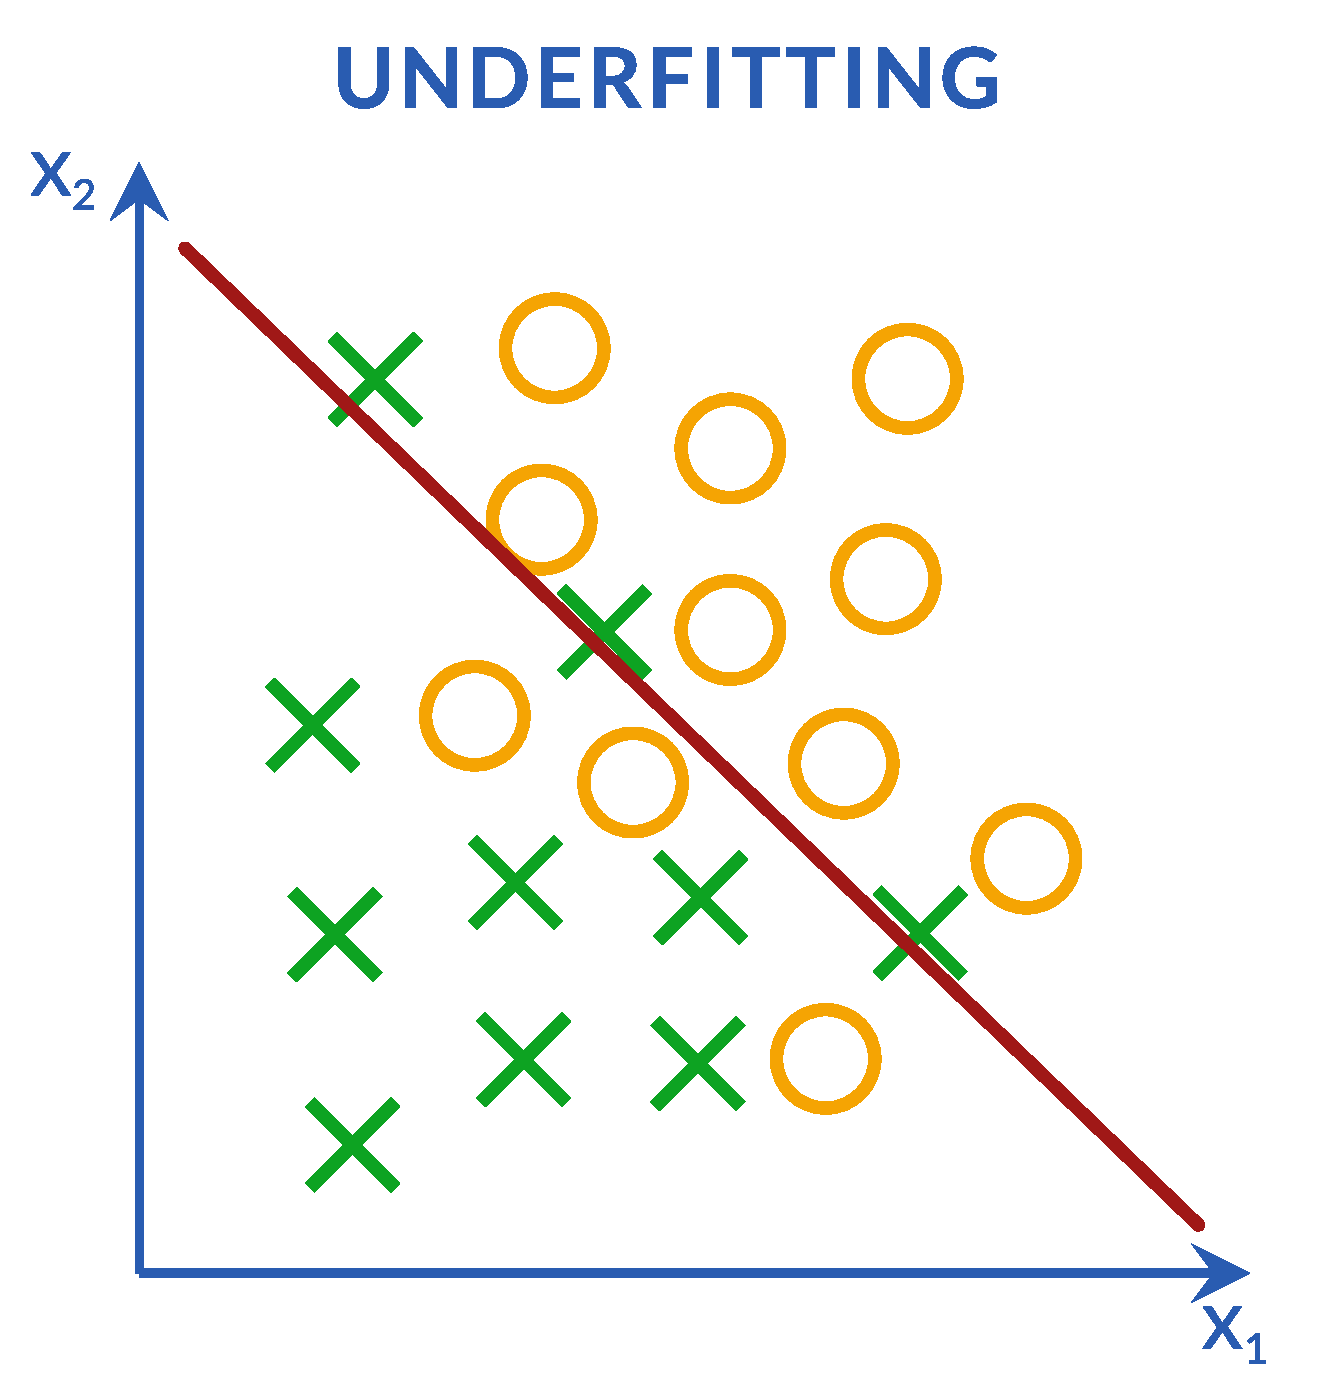
\includegraphics[width=\columnwidth]{figures/introduction/underfitting.pdf}
	\end{subfigure}%
	\begin{subfigure}{0.33\textwidth}
		\centering
		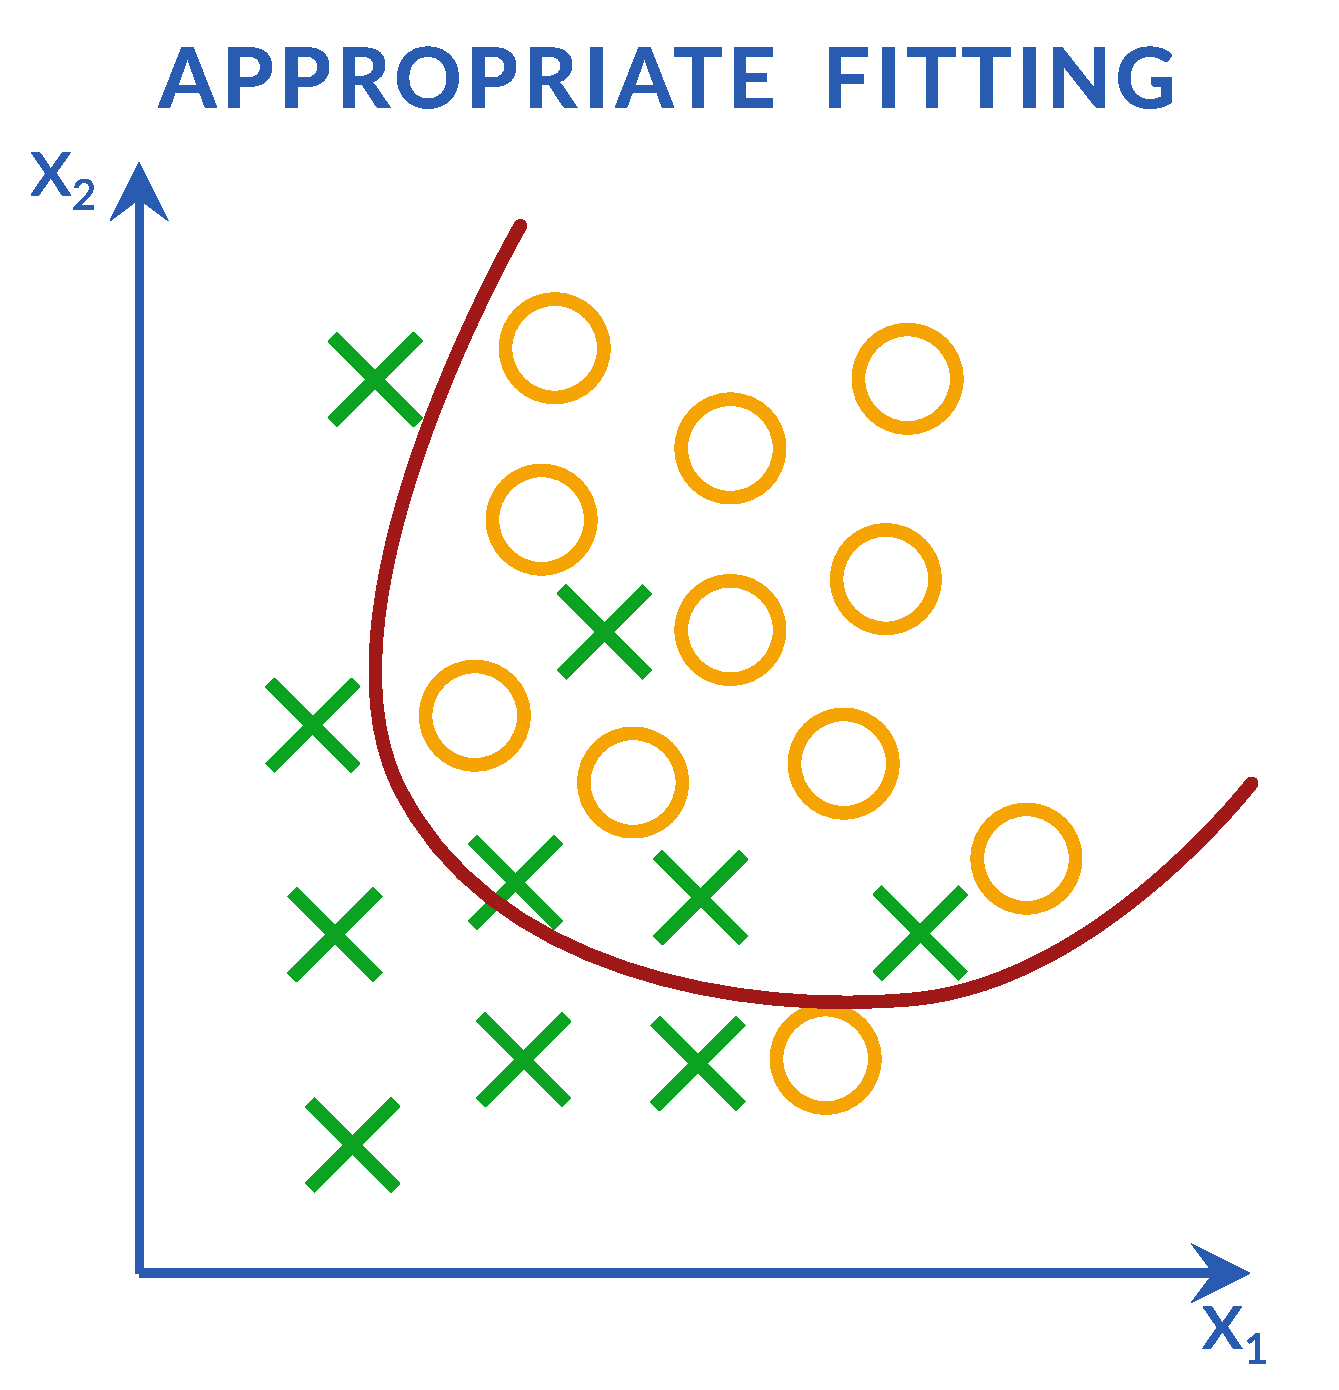
\includegraphics[width=\columnwidth]{figures/introduction/appropriate .pdf}
	\end{subfigure}%
	\begin{subfigure}{0.33\textwidth}
		\centering
		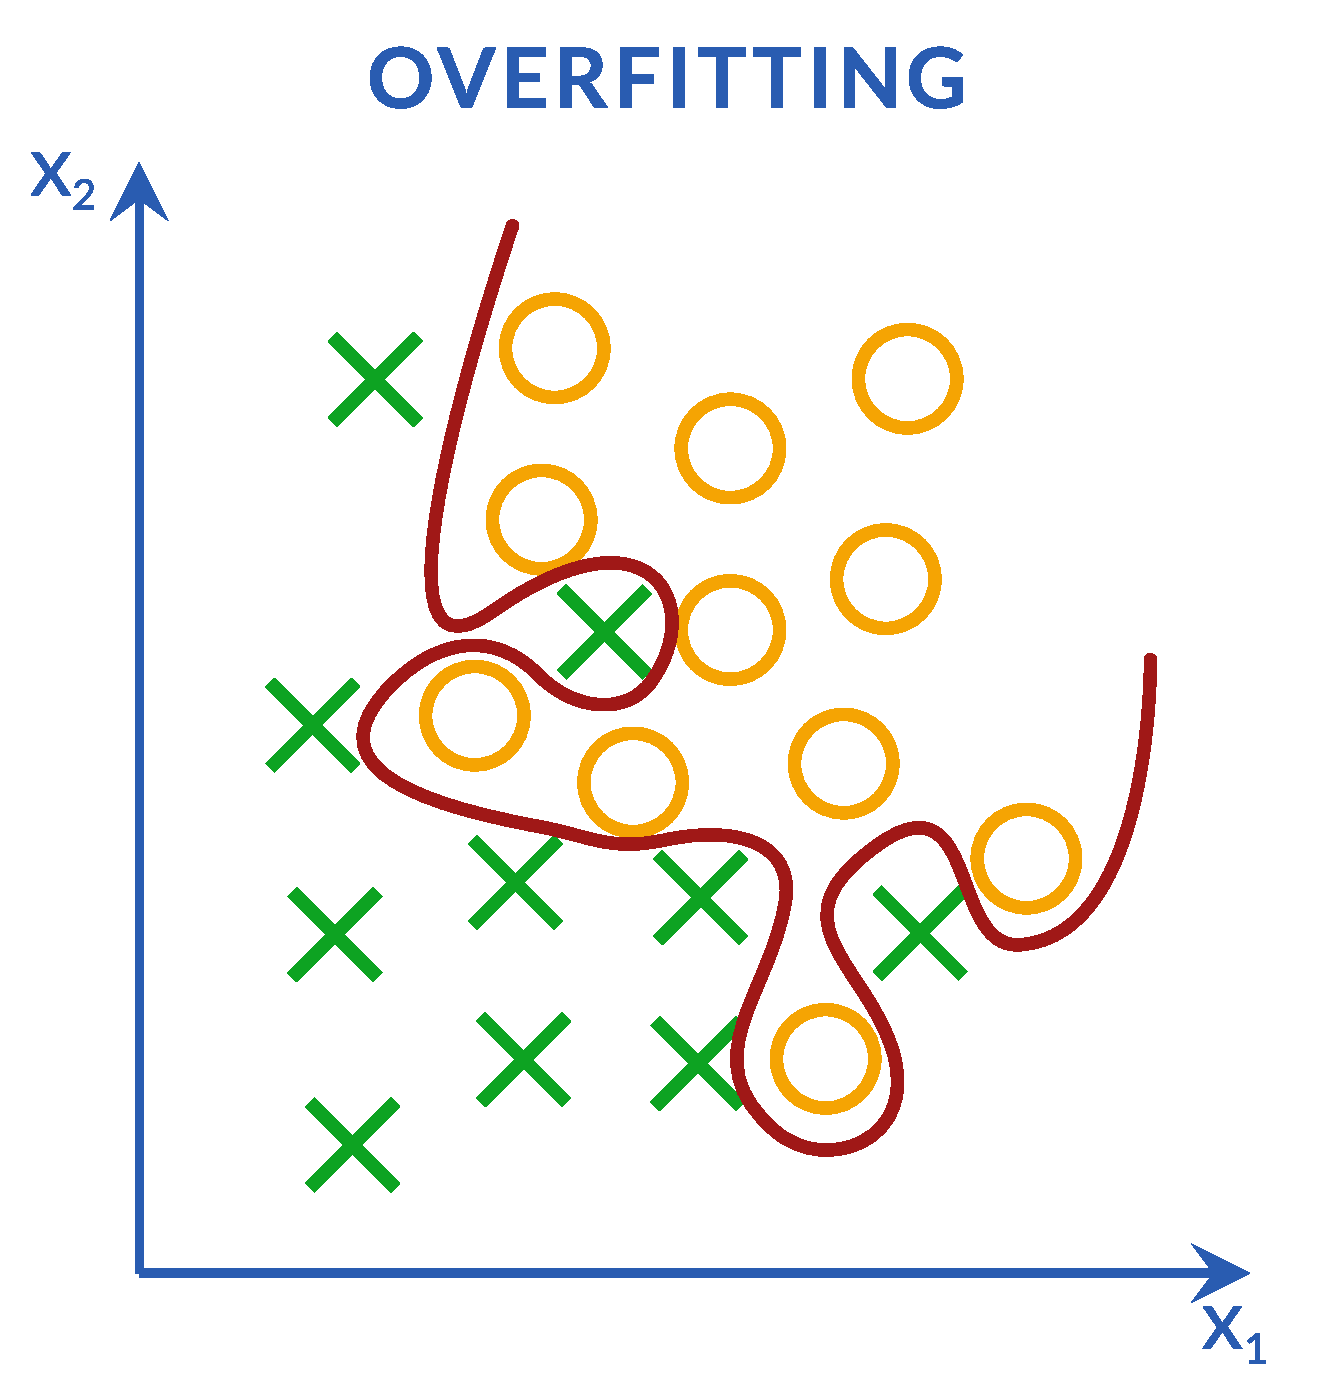
\includegraphics[width=\columnwidth]{figures/introduction/overfitting.pdf}
	\end{subfigure}
	\caption{Three different scenarios of model selection. On the left, the selected model does not have enough representational power to capture desired features in our data set. The center image model is complex enough to balance bias and variance while still being able to generalize on new data. We have a too-complex model for the given data set on the right. Too many parameters and the model will be able to capture all the features of the data, even the noise, leading to an inferior generalization.}
	\label{gr:fittingScenarios}
\end{figure}
\par
This principle can be nicely illustrated on an example of the MSE loss function and linear relation between input and target:
\begin{equation}
	y = f_{\vbtheta}(\vb{x}) + \epsilon \mathcomma
\end{equation}
where $\epsilon$ is a noise distributed according to a Gaussian distribution $\epsilon \sim \mathcal{N}(0, \sigma_\epsilon^2)$. In this case, the MSE loss function would be:
\begin{equation}
	\mathcal{L}_{\text{MSE}} = \sum_{i=1}^N (y_i - f(\vb{x_i}; \vbtheta))^2 \mathperiod
\end{equation}
Following the simple exercise in algebra and probability \cite{MLintro}, we can factor this loss into three individual components:

\begin{equation}
	\text{error} = \text{bias}^2 + \text{var} + \text{noise} \mathcomma
\end{equation}

where \textit{bias} is:

\begin{equation}
	\text{bias}^2 = \sum_{i=1}^N \left(f(\vb{x}_i) - \expval{f(\vb{x_i}; \hat{\vbtheta}_{\mathcal{D}})}_\mathcal{D}\right)^2 \mathcomma
\end{equation}

and \textit{variance}:

\begin{equation}
	\text{var} = \sum_{i=1}^N \expval{\left(f(\vb{x_i}; \hat{\vbtheta}_{\mathcal{D}}) - \expval{f(\vb{x_i}; \hat{\vbtheta}_{\mathcal{D}})}_\mathcal{D}\right)^2}_\mathcal{D} \mathperiod
\end{equation}

Bias represents how well our model would perform if we had an infinite amount of data, and the variance tells us how much our model fluctuates because of the finite amount of samples we have. Increasing the number of parameters will reduce the bias, but at some moment, the variance will increase. This is the central concept in ML, the trade-off between the complexity of a model and the amount of data we have to train it on. Because, in practice, we are usually presented with a limited amount of data. Choosing a less complex model with a higher bias will often lead to less variance and better generalization on new data points.
\par
Now that we have covered the basic intuition behind ML and DL, we will specify one simple model we will use later in the thesis, \textit{logistic regression}. Let us consider a case where our target variable $y$ can take a value $m = 0, \dots, M-1$ from one of the $M$ classes. We want to define a function that, given an input, returns a probability that it belongs to one of the $M$ classes. One such function is the \textit{sigmoid} function:
\begin{equation}
	\sigma(s) = \frac{1}{1 + \exp(-s)}
\end{equation}
Let us start first with a simple case of two classes $y_i = \{0, 1\}$. Then a probability that given data point $\vb{x}_i$ belongs to a category is:
\begin{align}
	p(y_i=1 | \vb{x}_i, \vbtheta) &= \frac{1}{1 + \exp(-\vb{x}_i^T \vbtheta)} \\
	p(y_i=0 | \vb{x}_i, \vbtheta) &= 1 - p(y_i=1 | \vb{x}_i, \vbtheta)
\end{align}
The most appropriate loss function would be cross-entropy:
\begin{equation}
	\mathcal{L}_{\text{BCE}} = -\sum_{i=1}^N y_i\log(\sigma(\vb{x}_i^T \vbtheta)) + (1-y_i)\log(1-\sigma(\vb{x}_i^T \vbtheta))
\end{equation}
We can minimize this loss function, but there is no simple closed-form solution and some of the minimization methods we have discussed need to be applied. Moving to a general case when instead of $2$, we have $M$ classes, and following one-hot encoding, we can write individual probabilities for each class as:
\begin{equation}
	p(y_{i,m'}=1|\vb{x}_i, \{\vbtheta\}_{k=0}^{M-1}) = \frac{\exp(-\vb{x}_i^T \vbtheta_{m'})}{\sum_{m=0}^{M-1}\exp(-\vb{x}_i^T \vbtheta_m)}
\end{equation}
This is known as \textit{SoftMax} function, and the appropriate cross-entropy is:
\begin{align}
	\mathcal{L}_{\text{CCE}} = &-\sum_{i=1}^N \sum_{m=0}^{M-1} y_{i,m} \log(p(y_{i,m}=1|\vb{x}_i, \vbtheta_m)) \nonumber \\ &+ (1-y_{i,m})\log(1 - (p(y_{i,m}=1|\vb{x}_i, \vbtheta_m)))
\end{align}
\subsection{Neural networks for ML}
Models that we have considered so far are simple ML models that form a basis for any further improvements. The introduction of neural networks catapulted the field of ML and DL to the heights of today. 
\begin{figure}[H]
	\centering
	\begin{subfigure}[c]{0.5\textwidth}
		\centering
		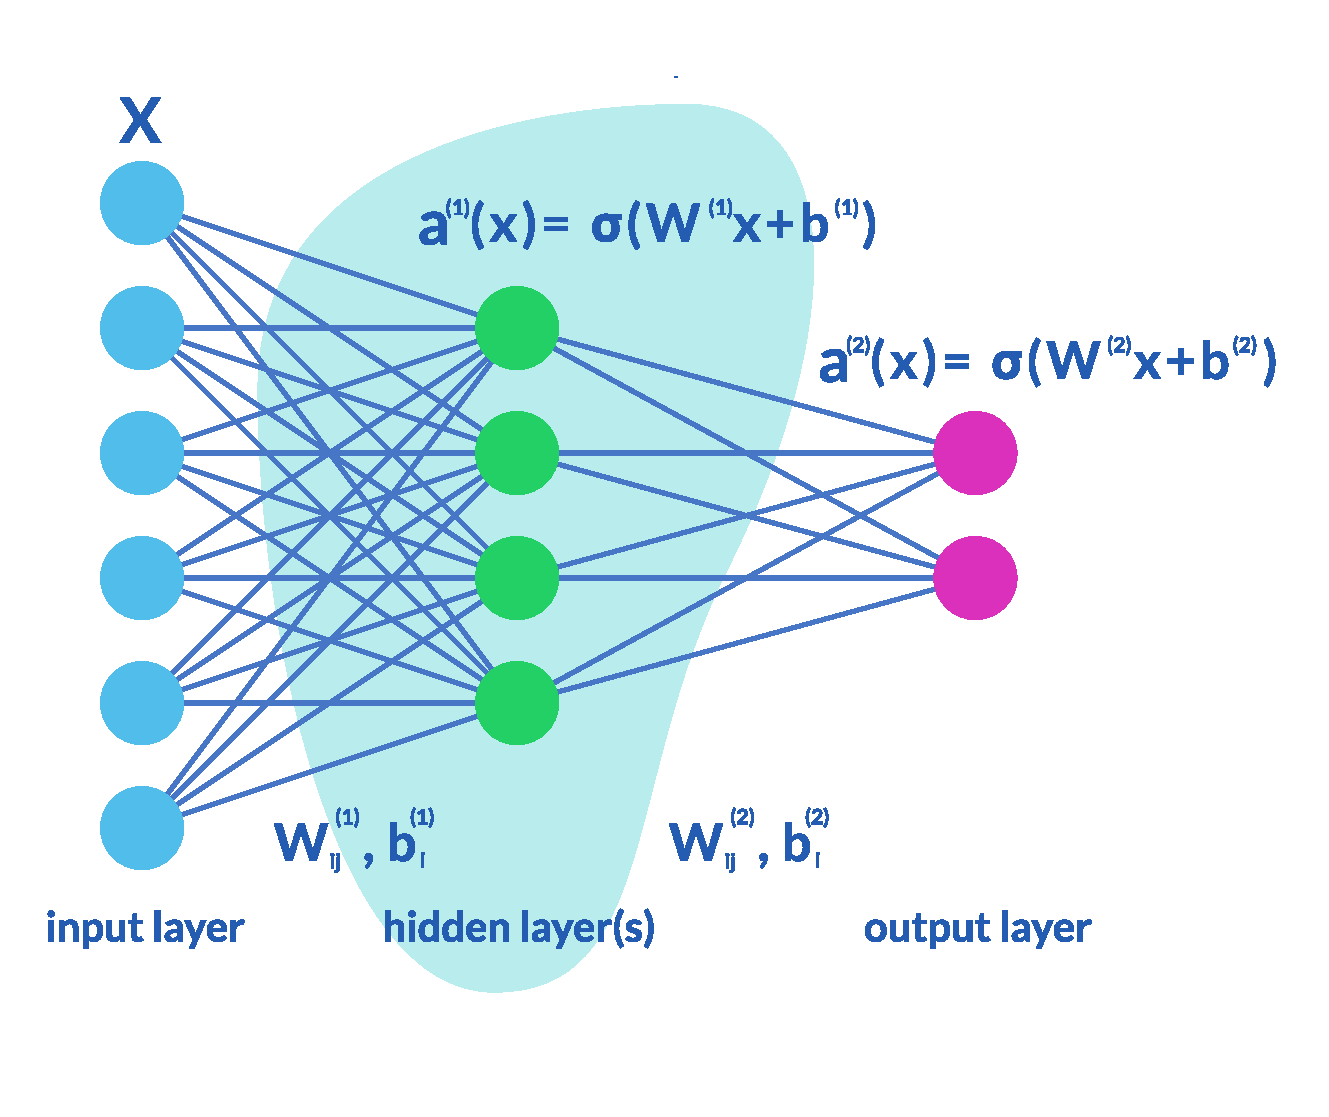
\includegraphics[width=\columnwidth]{figures/introduction/neuralNetwork.pdf}
	\end{subfigure}%
	\begin{subfigure}[c]{0.5\textwidth}
		\centering
		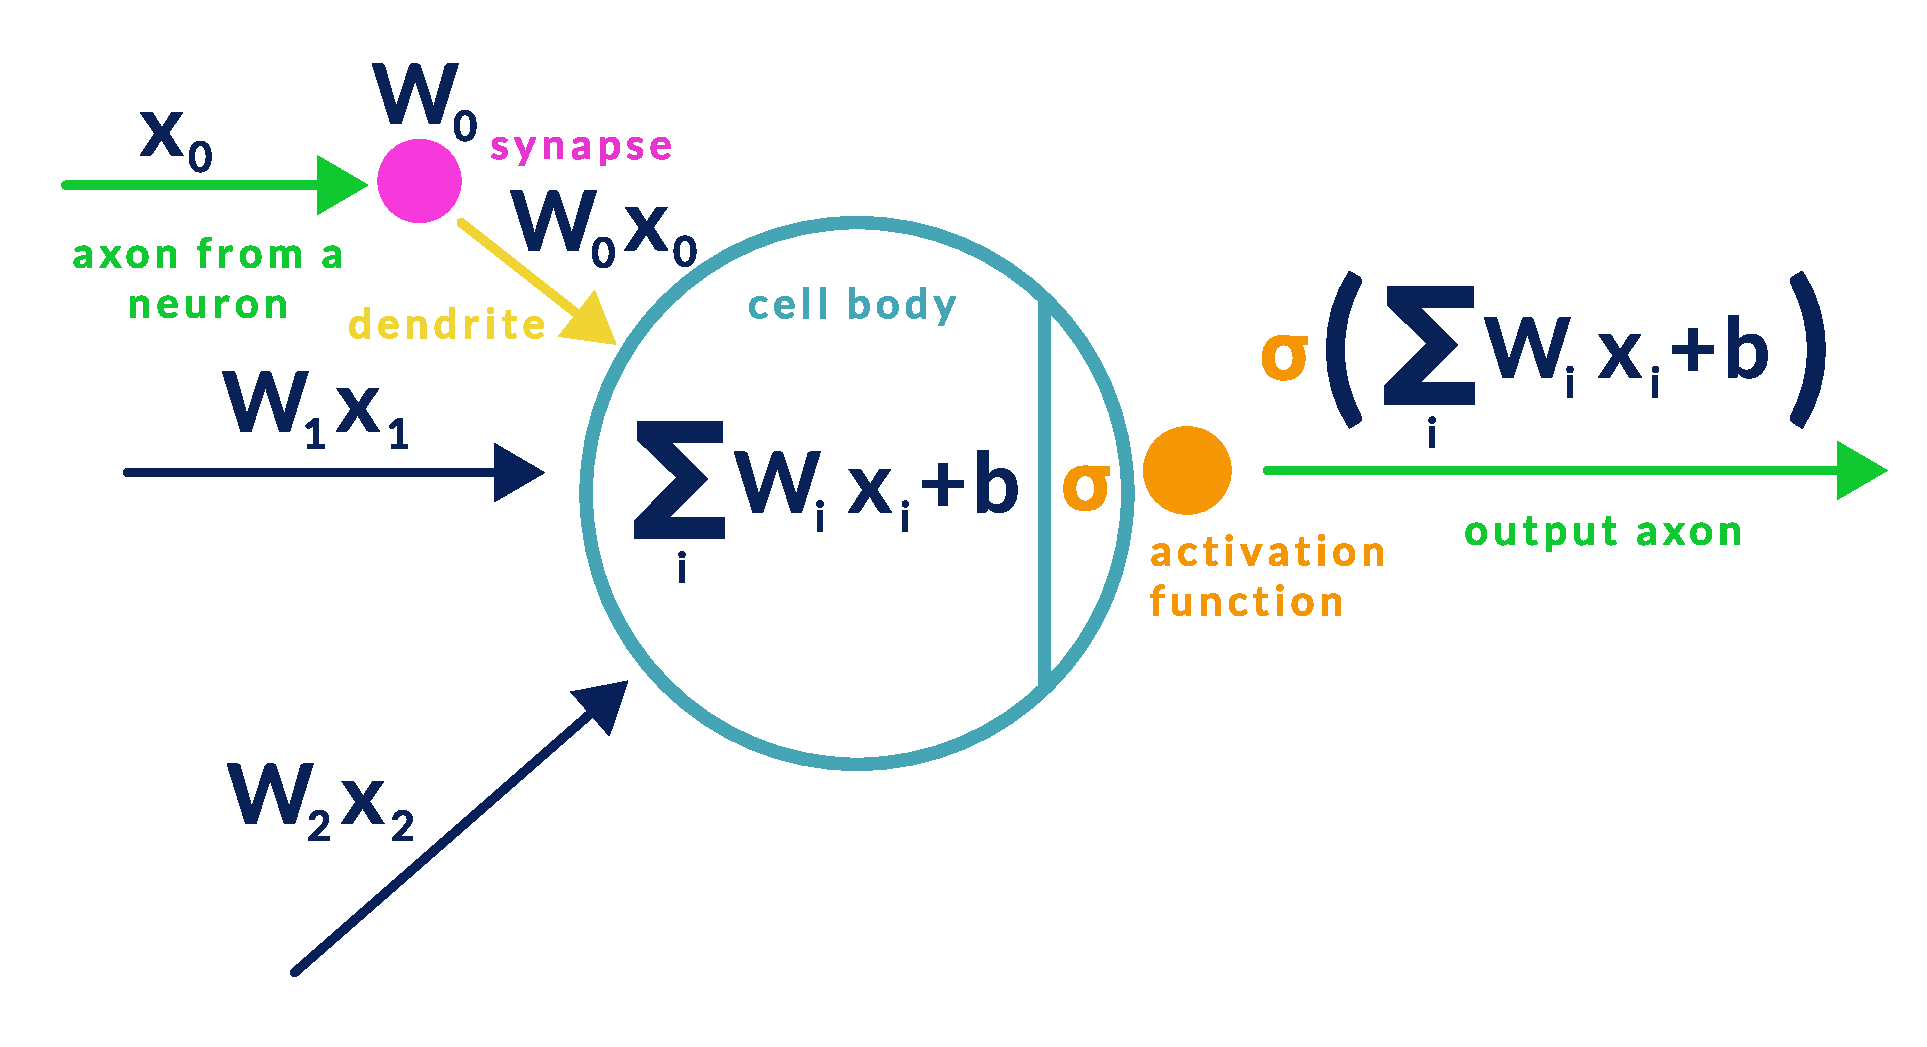
\includegraphics[width=\columnwidth]{figures/introduction/neuron.pdf}
	\end{subfigure}
	\caption{On the left is an illustration of a fully connected neural network with a single hidden layer and two layers in total. On the right is a neuron, an elementary building block of neural networks.}
	\label{gr:neuronNetwork}
\end{figure}
The fundamental building element of a neural net is a neuron $i$, Fig.(\ref{gr:neuronNetwork}) that takes as an input $d$ dimensional vector of features $\vb{x} = (x_1, x_2, \dots, x_d)$ and produces a scalar output $a_i(\vb{x})$. A neural network is formed by stacking many neurons on top of each other to form a single layer. Then multiple layers are stitched together to form the whole network. Stacking multiple layers enhances our neural networks' expressivity, which helps us approximate complex functions. The existence of a universal approximation theorem states that a neural network with a single layer can approximate any "nice" and continuous function with arbitrary accuracy. The first layer is called an input layer, the last layer is called an output layer, and any layer(s) in-between is(are) called hidden layer(s). What makes neural networks work is an introduction of some non-linearity between layers, \textit{activation function}. We usually take the same activation function for all the neurons in a single layer. Going from one to the other layer, first, the linear transformation of the form is computed: 
\begin{equation}
	z^i = \vbomega^i \cdot \vb{x} + \vb{b}^i = \vb{x}^T \cdot \vb{w}^i \mathcomma
\end{equation}
where weight vector $\vbomega^i = (\omega_1^1, \omega_2^1, \dots, \omega_d^1)$, $\vb{x}=(1, \vbx)$ and $\vb{w}^i = (b^i, \vbomega^i)$. After the linear transformation, the activation function is applied to get a post-activation value of a layer:
\begin{equation}
	a_i(\vb{x}) = \sigma_i(z^i)
\end{equation}
There are many possibilities for activation functions; some of the popular ones are step-function, sigmoid, hyperbolic tangent, rectified linear units (ReLUs), leaky rectified linear units (leaky ReLUs), and exponential linear units (ELUs)\cite{MLintro}. What we choose as an activation function will impact the performance of our network and greatly depend on a specific task we are trying to solve, which we will later see in Chapter \ref{ch:edgeofchaos}. Another consideration should be taking a derivative of activation functions as they are required for any gradient-based function minimization methods.
\par
If we remember from our previous sections how to train a network, we will need to find a derivative of a loss function with respect to all the weights for any gradient-based method. At first, this seems like a daunting task. However, luckily, there is a very nice and elegant algorithm that can help us find all of the desired derivatives easily, \textit{backpropagation}. Behind the fancy name is nothing more complicated than a simple chain rule for differentiation. Because this is crucial background knowledge to the chapter, we discuss it here. In order to fully understand this backbone of an algorithm, let us set the stage first. We will take a network with $L$ layers labeled with $l=1,\dots, L$. Weights $\omega^l_{j,k}$ connect $k$-th neuron from $l-1$ layer to a $j$-th neuron in layer $l$. The bias associated with this neuron is $b_j^l$. Then we can write a post-activation value $a_j^l$ of this neuron as:
\begin{equation}
	a_j^l = \sigma \left(\sum_k \omega^l_{j,k}a_k^{l-1} + b_j^l\right) = \sigma(z_j^l)
	\label{eq:postactivation}
\end{equation}
where the linear combination part, the pre-activation value, is defined as:
\begin{equation}
	z_j^l = \sum_k \omega^l_{j,k}a_k^{l-1} + b_j^l
	\label{eq:linearInput}
\end{equation}
Let us think about how we compute the loss function. Directly the value of a loss function depends on the post-activation values $a_j^L$ from $L$-th layer, but these values indirectly depend on the post-activations from the previous layers. This is the crucial observation to set up a backpropagation algorithm. Define the error $\Delta_j^L$ of $j$-th neuron in the final $L$-th layer as a partial derivative of the loss function with respect to the weighted input $z_j^L$:
\begin{equation}
	\Delta_j^L = \pdv{\mathcal{L}}{z_j^L}
\end{equation}
Analogous to this, we can define the error for any neuron $j$ in arbitrary layer $l$ as:
\begin{equation}
	\Delta_j^l = \pdv{\loss}{z_j^l} = \pdv{\loss}{a_j^l}\sigma'(z_j^l)
	\label{eq:firstBackprop}
\end{equation}
we can also make the chain rule different in order to get the following:
\begin{equation}
	\Delta_j^l = \pdv{\loss}{z_j^l} = \pdv{\loss}{b_j^l}\pdv{b_j^l}{z_j^l} = \pdv{\loss}{b_j^l}
	\label{eq:secondBackprop}
\end{equation}
where we have used Eq.(\ref{eq:linearInput}) to find $\pdv{b_j^l}{z_j^l}=1$. As we stated before, the layered structure of the network ensures that the layer error $l+1$ depends on the post activations from layer $l$, and we can use the chain rule to expand:
\begin{equation}
	\begin{split}
		\Delta_j^l &= \pdv{\loss}{z_j^l} = \sum_k \pdv{\loss}{z_k^{l+1}} \pdv{z_k^{l+1}}{z_j^l} \\
		&= \sum_k \Delta_k^{l+1} \pdv{z_k^{l+1}}{z_j^l} \\
		&= \left(\sum_k \Delta_k^{l+1}\omega_{k,j}^{l+1}\right)\sigma'(z_j^l)
	\end{split}
	\label{eq:thirdBackprop}
\end{equation}
The final equation is:
\begin{equation}
	\pdv{\loss}{\omega_{j,k}^l}=\pdv{\loss}{z_j^k}\pdv{z_j^k}{\omega_{j,k}^l} = \Delta_j^l a_k^{l-1}
	\label{eq:fourthBackprop}
\end{equation}
Now we have all the necessary ingredients to state the entire backpropagation algorithm:
\begin{algorithm}[H]
	\caption{The backpropagation algorithm}
	\begin{algorithmic}[1]
		\State Calculate the post-activation values of all neurons in the input layer $a_j^1$
		\State Now using Eq.(\ref{eq:postactivation}) compute all the $z^l$ and $a^l$ values until the last layer
		\State Calculate the error of the final layer using Eq.(\ref{eq:firstBackprop}); for this, we will need to compute the analytical form of loss and activation functions manually
		\State Using Eq.(\ref{eq:thirdBackprop}) we can propagate error backwards in order to calculate $\Delta_j^l$
		\State The final step is using Eqs.(\ref{eq:secondBackprop}, \ref{eq:fourthBackprop}) in order to calculate the desired derivatives $\pdv{\loss}{w_{j,k}^{l}}$ and $\pdv{\loss}{b_j^l}$
	\end{algorithmic}
\end{algorithm}
The name backpropagation now makes sense; we are using a single forward pass through the network to compute linear combinations and post-activations, and then by backtracking through the network, we compute all of the derivatives. This specific nature of backpropagation makes it highly efficient when implemented on modern GPU units. The immediate relevance to the work in this thesis is the appearance of $\sigma'$ in Eq.(\ref{eq:postgeneral}). A core part of chapter \ref{ch:edgeofchaos} is the exploration of the effects of saturation, domain regions where $\sigma'=0$ and therefore negligible gradients, on the final training efficiency.
\subsection{Neural quantum states}
In order to motivate this next class of neural networks, we use some topics from quantum mechanics to guide us. Let us say that we have an isolated quantum system of spins $1/2$ in a chain of length N. Then we can expand any wave function in some arbitrary basis that will have $2^N$ coefficients. For example, consider a $1D$ system with $40$ spins. Directly writing down all the coefficients alone would be an infeasible task; there are $2^40 \sim 10^12$ different coefficients, and just writing them down would take up more than $40$TB of space. If we want to study real-life systems with many more particles and in many more dimensions like $2D$ or $3D$, we need to find some other methods of doing it. This should not be the end; usually, only a small part of a Hilbert space is of relevance, and this fact can help us a lot. We can apply some of the \textit{variational methods} that try to find the optimal representation of the quantum state, one that will encompass all the necessary features and be computationally friendly. We can write the basis expansion as:
\begin{equation}
	\ket{\Psi_{\vbtheta}} = \sum_{s=1}^{2^N} \Psi_{\vbtheta}(\vb{s})\ket{s}
\end{equation}
where $\Psi_{\vbtheta}(\vb{s}) = \braket{s}{\Psi_{\vbtheta}}$ and our goal would be to find the best $\Psi_{\vbtheta}(\vb{s})$ that approximate a ground state but $\text{dim}[\vbtheta] \ll \text{dim}[s]$. We can then use this proposed model for the wave function to compute the expectation values of desired operators in polynomial time. To cast the usual complex wave function computations in terms of probabilities, we use the following local estimator method to compute the expectation value of some arbitrary operator $\hat{O}$ \cite{MLintro}:
\begin{equation}
	\begin{split}
		\expval{\hat{O}} &= \frac{\ev{\hat{O}}{\Psi_{\vbtheta}}}{\braket{\Psi_{\vbtheta}}} \\
		&=\frac{\sum_{s,s'} \braket{\Psi_{\vbtheta}}{s} \mel{s}{\hat{O}}{s'}\braket{s'}{\Psi_{\vbtheta}}}{\sum_s |\braket{\Psi_{\vbtheta}}{s}|^2} \\
		&= \frac{\sum_s |\braket{\Psi_{\vbtheta}}{s}|^2 \sum_{'s}\mel{s}{\hat{O}}{s'}\frac{\braket{s'}{\Psi_{\vbtheta}}}{\braket{s}{\Psi_{\vbtheta}}}}{\sum_s |\braket{\Psi_{\vbtheta}}{s}|^2}
	\end{split}
\end{equation}
We can identify two terms here:
\begin{align}
	p(\vb{s}) &= \frac{|\braket{\Psi_{\vbtheta}}{s}|^2}{\sum_s |\braket{\Psi_{\vbtheta}}{s}|^2} \\
	O_{\text{loc}}(s) &= \sum_{s'} \mel{s}{\hat{O}}{s'}\frac{\braket{s'}{\Psi_{\vbtheta}}}{\braket{s}{\Psi_{\vbtheta}}}
\end{align}
The first is the usual quantum mechanics probability density. The second one $O_{\text{loc}}(\vb{s})$ is called a \textit{local estimator} of $\hat{O}$. Therefore we can write a quantum mechanical expectation as a classical expectation value:
\begin{equation}
	\expval{\hat{O}} = \sum_s p(\vb{s}) O_{\text{loc}}(\vb{s}) = \expval{O_{\text{loc}}(\vb{s})}_p
	\label{eq:varexpval}
\end{equation}
The procedure of how to estimate the expectation value of any operators in the form of Eq.(\ref{eq:varexpval}) is very reminiscent of Eq.(\ref{eq:mcestimation}) so we can write it as:
\begin{equation}
	\expval{\hat{O}} \approx \frac{1}{N_{\text{samp}}} \sum_{i=1}^{N_{\text{samp}}} O_{\text{loc}}(\vb{s}^i)
	\label{eq:explocalop}
\end{equation}
Now we are back to the conventional statistical physics that we reviewed earlier. We now know how to compute this by constructing a Markov Chain and using Monte Carlo simulation to compute the expectation value.
\par
What remains is to make a suitable variational ansatz $\Psi_{\vbtheta}(\vb{s})$. This is where we combine ML with Monte Carlo, an insight from Carleo and Troyer \cite{carleoTroyer}. We will use the \textit{restricted Boltzmann machines} (RBM) for this job. Neural network architecture is called the \textit{neural quantum state} (NQS). 
\begin{figure}[H]
	\centering
	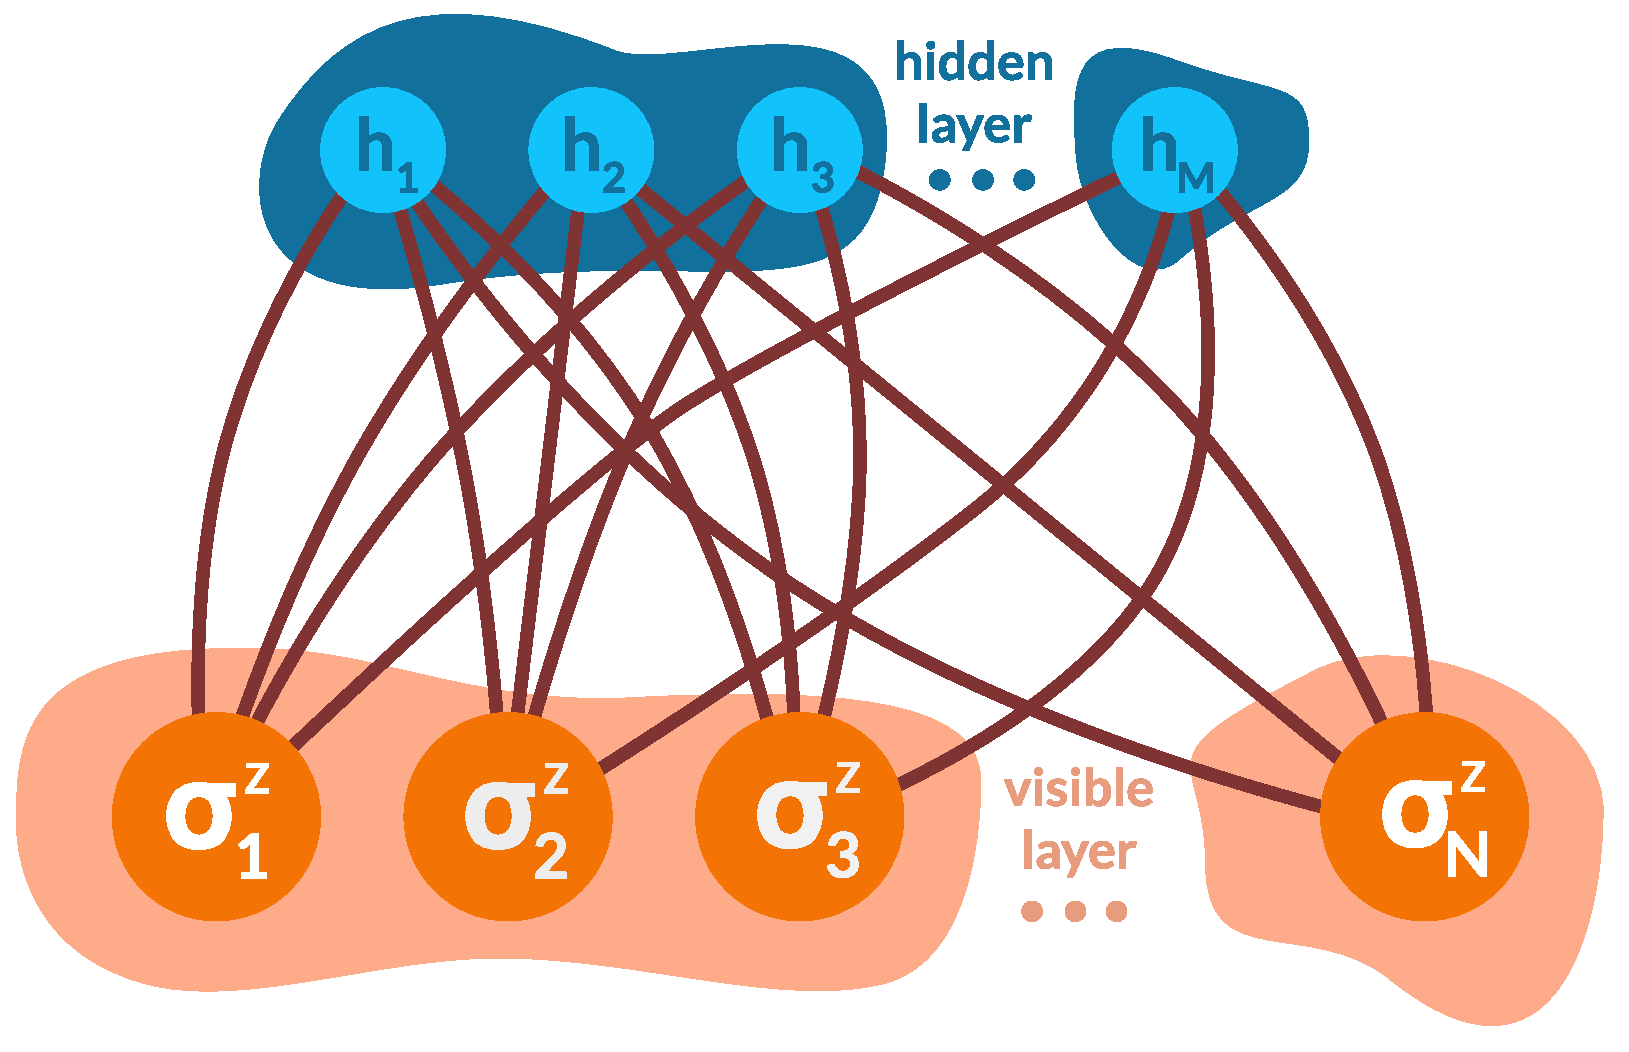
\includegraphics[width=8cm]{figures/introduction/rbm.pdf}
	\caption{Illustration of a restricted Boltzmann machine (RBM) neural network. We use RBM as a variational ansatz to represent a wave function of $N$ spins with $s = (\sigma_1^z, \sigma_2^z, \dots, \sigma_N^z)$ and $M$ hidden units $h = (h_1, h_2, \dots, h_M)$. There is general proof that a sufficiently dense ($\alpha \gg 1$) RBM can approximate any probability distribution \cite{HORNIK1989359}.}
	\label{gr:rbmArchitecture}
\end{figure}
RBM networks are fully connected two-layer networks with one visible and one hidden layer. The visible layer has $N$ spins, and the hidden layer has $M$ spins. We will label the ratio of the number of hidden vs. visible neurons as $\alpha = \frac{M}{N}$. The insight of Carleo and Troyer was that the intrinsically non-local correlations of RBM could lead to a significantly more compact representation of many-body quantum states. Then the ansatz wave function is given by:
\begin{equation}
	\Psi_{\vbtheta}(\vb{s}) = \sum_h \exp(\vb{b}_v^\dagger \cdot \vb{s} + \vb{b}_h^\dagger \cdot \vb{h} + \vb{h}^\dagger  \vb{W} \vb{s} ) \mathperiod
\end{equation}
Because of the network architecture, we can trace out hidden variables and get the following:
\begin{equation}
	\Psi_{\vbtheta}(\vb{s}) = \exp(\vb{b}_v^\dagger \cdot \vb{s}) \prod_{i=1}^{M}2\cosh(\vb{b}_{h,i} + \vb{W}_i \cdot \vb{s}) \mathcomma
\end{equation}
where  $\vb{b}_{h,i}$ and $\vb{W}_i$ are $i$-th hidden bias and weight matrix row. Now we have a model wave function that will convert our spin configuration into a desired probability.
\par
With this ansatz, we are back in familiar territory to find the ground state energy of some Hamiltonian:
\begin{equation}
	E(\vbtheta) = \ev{\hat{H}}{\Psi_{\vbtheta}} \mathcomma
\end{equation}
in terms of ML, this will be our loss function. We must also remember that this variationally obtained ground state energy is $E(\vbtheta) \geq E_0$, but this is strictly true when expectation values are calculated exactly.
\newline
We can exchange operator $\hat{O}$ for the energy in Eq.(\ref{eq:explocalop}) in order to get stochastically approximated energy:
\begin{equation}
	E(\vbtheta) \approx \frac{1}{N_{\text{samp}}} \sum_{i=1}^{N_{\text{samp}}} E_{\text{loc}}(\vb{s}^i)
\end{equation}
where we have defined our local energy as $E_{\text{loc}}(\vb{s}) = \sum_{s'}\ev{\hat{H}}{s}\frac{\braket{s'}{\Psi}}{\braket{s}{\Psi}}$. We will use gradient-based optimization methods to minimize our loss function. The energy gradient with respect to parameters is:
\begin{equation}
	\pdv{E(\vbtheta)}{\theta_i} = 2\Re \left[\expval{E_{\text{loc}}(\vb{s}) O_i^\star (\vb{s})} - \expval{E_{\text{loc}}(\vb{s})}\expval{O_i^\star (\vb{s})}\right]
	\label{eq:rbmDeriv}
\end{equation}
where $\theta_i$ is the $i$-th parameter and operator $\hat{O}_i$ is defined as:
\begin{equation}
	O_i(\vb{s}) = \pdv{\theta_i}\log \braket{s}{\Psi_{\vbtheta}} = \ev{\hat{O}_i}{s}
\end{equation}
Now we have all the necessary ingredients to formulate the final algorithm for finding the ground state of a Hamiltonian $\hat{H}$ using RBM and variational method:
\begin{algorithm}
	\caption{Finding ground state with NQS}
	\begin{algorithmic}
		\State Randomly initialize all the parameters of a neural network $\vbtheta$
		\For{$i = 1$ to $N_{\text{steps}}$}
		\State Generate $N_{\text{samp}}$ samples using Markov chain
		\State Calculate the gradient of the energy $\pdv{E(\vbtheta)}{\theta_i}$ using Eq.(\ref{eq:rbmDeriv})
		\State Update parameters using SGD or some other minimization technique
		\EndFor
		\State \Return Optimized parameters $\hat{\vbtheta}$
	\end{algorithmic}
\end{algorithm}
\par
Compared to the current standard numerical methods, NQS can have the same or better accuracy\cite{carleoTroyer}. Compared with MPS, PEPS, and DMRG for transverse-field Ising (TFI) and anti-ferromagnetic Heisenberg models (AFH), NQS achieved better accuracy for sufficiently large $\alpha$ ration. AFH, when compared to DMRG, NQS with $\alpha=4$ managed to outperform DMRG with the bond dimension of $\sim 160$, pointing towards a much more compact representation of a many-body wave function. This also has practical implications, as fewer variational parameters are easier to optimize. Even when applied at the critical point, NQS managed to get the accuracy of the state-of-the-art methods or even better, albeit with slowed down converged, which is expected near the criticality. The compact nature and ability to express the wave function near the critical point prompted us to use it to analyze entanglement entropy for lattice gauge fields explored in chapter \ref{ch:EE} of the thesis. 
\newpage

\section{This thesis}
In the introduction, we have covered the basic ideas used later in this thesis. We started with introductory topics in thermodynamics and statistical physics, then moved to a basic introduction to Monte Carlo methods and all the required knowledge to understand our physical system's simulation design and analyze the results. The proceeding section was dedicated to the basics of machine learning, deep learning, and appropriate selection of model, loss function, and minimization method. The last section culminated in a synergy of the previously mentioned topics by combining quantum physics, Monte Carlo methods, and neural networks in neural quantum states that we used to find the ground state and its energy of lattice gauge theories.

\subsection{Chapter 1 - Thermalization in quantum systems}
The properties of closed unitary quantum systems and how they exactly thermalize have been one of the leading research questions in statistical physics for a long time. The puzzle is that a thermal ensemble is formally a mixed state, but a mixed state can never arise from unitary evolution from a pure state. The usual answer to how they thermalize is the eigenstate thermalization hypothesis (``ETH'') \cite{srednickiETF}. The hypothesis is that in generic quantum theory with many degrees of freedom, most observables will have a particular form of matrix elements after averaging, and observable will \textit{appear} to thermalize. However, recently \cite{OTHpaper} showed that ETH has to be taken with care. Even in free field theory, there are operators that \textit{appear} to relax, called operator thermalization hypothesis (OTH). Given a particular no-go condition, the retarded Green's function will typically decay exponentially unless the condition is met. Finding an operator that will satisfy this condition in a general non-integrable theory is challenging but possible. On the other hand, this job is more straightforward in integrable theories due to the extensive number of conserved quantities. We work in the transverse field Ising (TFI) model where we compare a specially designed operator $\Gamma$ that will satisfy the no-go condition with the Pauli $\sigma^z$ operator that does not satisfy it. Through the examples, we show the differences and similarities of ETH and OTH and how, despite TFI being an integrable theory, $\sigma^z$ will relax after the perturbation. Also, we have demonstrated how the no-go condition is a feature of integrability, and any minor deviation from integrability will cause $\Gamma$ to relax. Our results were later confirmed in \cite{likeOurETH}.  

\subsection{Chapter 2 - Symmetry restoration through ``registry''}
Starting from the simple Wegner gauge theory \cite{Wegner,Kogut}, Fradkin and Shenker \cite{Fradkinshenker} discovered that when an added matter field is ``in the fundamental'', meaning that there is an additional Higgs field that is also governed by $Z_2$ symmetry as the gauge fields, the Higgs phase and confining phase become one, without a phase transition. In this chapter, we propose a straightforward generalization of their lattice gauge theory that could serve as a candidate for a highly entangled state of matter. We will consider adding multiple $Z_2$ and $O(N)$ matter fields on the lattice and gauging them with a common $Z_2$ field. It will be shown how, in such a case, the Higgs phase becomes separate from the confining phase. It will be characterized by the ``registry'' order parameter, which turns out to be gauge invariant $p=2^{N_{\text{rep}-1}}$ Potts type symmetry, where $N_{\text{rep}}$ is the number of matter field copies. Interpretation for this type of symmetry is that different matter copies align their vectors locally in strictly parallel or anti-parallel ways, even in the case of continuous $O(N)$ matter fields. These theories will be studied using Monte-Carlo simulation on a $3D$ grid using the Metropolis-Hastings algorithm and annealing techniques to improve the convergence near the critical point. From the simulation results, we can discover some unidentified ``pseudo-universality'' associated with the form of the phase diagram for various numbers of matter field theories.

\subsection{Chapter 3 - Entanglement entropy of lattice gauge theories}
Building further on the work from the previous chapter, we will study entanglement entropy in the neural network representation of the above lattice gauge theories, now considered as quantum theories in one lower dimension. Following the seminal work of Carleo and Troeyer \cite{carleoTroyer}, we will construct neural quantum states as the representation of our theory using a variational wavefunction based on Restricted Boltzmann Machines used in Machine Learning. Using ideas from tensor networks that the bond dimension represents the upper bound on the amount of entanglement a state can have, we will postulate that by increasing the number of matter fields, ground state entanglement entropy of our lattice gauge theory will increase as the ratio of hidden vs. visible nodes. We have tested our hypothesis in the case of $2, 3$, and $4$ matter fields. Within the achievable computational limits, the results are puzzling. Even though increasing the number of variational parameters improved the energy of the ground state, the impact on the entanglement entropy is less than obvious. Curves of entanglement entropy for different system sizes look the same up to the statistical errors. 

\subsection{Chapter 4 - Phase space and efficient learning of deep neural networks}
This chapter combines some statistical physics insights into machine learning with the computational mechanics of deep random feedforward neural networks. In recent times with the ever-growing amount of available data, neural networks have become one of the de-facto methods for analyzing and processing vast amounts of data \cite{Mehta_2019}. One of the reasons why these methods became so popular is their ability to express any function with a relatively small number of parameters \cite{MLintro} and the ease with which this \textit{expressivity} can be increased by adding more depth. This easy fix does not come for free; deep neural networks generally require more training computations. Specifically, they suffer from exploding or vanishing derivatives in optimizing the parameters. The phase space of deep random feedforward neural networks is characterized by the variance of initial weights and the variance of initial bias. Following previous work \cite{arxiv.1606.05340,2016arXiv161101232S} that demonstrated the existence of order-to-chaos regime change in this phase space, we will examine the behavior of the pre-and post-activations in terms of their distributions and also final accuracy on classification task such are MNIST and CIFAR10. The phase boundary dividing these two regimes is called the edge of chaos (EOC). We demonstrate that for the $\tanh$ activation function, not all points along the EOC yield the same learning efficiency. In the case of shallow and narrow neural networks, we define the line of uniformity (LOU), a set of points for which the final layer post-activation values are distributed uniformly, i.e., with maximal entropy. We show that moving away to the right from LOU and drastically increasing initial variances means that gradient saturation will start impeding optimization over parameters, i.e., the learning process.    
